
\usepackage[labelformat=simple,listofformat=subsimple]{subfig}
\usepackage{longtable}
\usepackage[boxed]{algorithm2e}
\usepackage{makecell}
\usepackage{rotating}
\usepackage{wrapfig}
\usepackage{tikz}
\usepackage{forest}
\usepackage{pgfplots}
\usepackage{multirow}
\usepackage{verbatim}
\usepackage{listings}

\pgfplotsset{compat=1.6}

\lstset{language={C++}}

\AtBeginDocument{
	\setcounter{tocdepth}{0}
}

\setcounter{totalnumber}{100}

\newcommand{\DMC}{死人的宝箱}
\newcommand{\FM}{造雾机}
\newcommand{\Grate}{格栅}
\newcommand{\PL}{等离子灯}
\newcommand{\Volcano}{火山}
\newcommand{\GC}{高尔夫球洞}
\newcommand{\Lesion}{损伤}
\newcommand{\Bamboo}{竹}


\input{preamble}
\input{ids}

\title{
	\includegraphics[width=0.7\textwidth]{figure/terraria.png}\\
	电路文档\\
	v3.3.3
}

\author{putianyi888}
\date{
	\today\\
	项目地址 \github{putianyi888/TerrariaWiringTutorial}
}

\begin{document}

\maketitle
\tableofcontents

\mainmatter
\hypersetup{pageanchor=true}

\chapter{从零开始}

\section{前言}\label{sec1:1}
\begin{note}{}{}
本书初编写时的游戏是1.3.5.3版本。1.4更新后我们正在努力学习新的内容并更新。
\end{note}

本书定位为“文档”,主要用于系统性收录电路理论,因此行文中会先讲理论后讲例子。如果读者觉得理论难以理解,不妨先看例子,再结合例子看理论。

每章后的思考题,有部分是经典电路的分析理解,有部分是因为我懒而没有去做的电路,还有一部分是纯理论推导。它们的共同点就是做不做都无所谓。与思考题相比,正文中用于举例、自成一节的电路是必须熟练掌握的。

学习\nameref{dianlujichu}后,你就可以做出大多数解谜地图与刷怪场里的电路,包括南瓜神教等。学习\nameref{sec7}后,你将可以研究设计复杂电路,例如电路小游戏。\nameref{chap7}难度较高,仅供有能力的读者阅读。不要忽视附录,附录中包含大量的优秀作品和教程的链接,它们会拓宽你的想象力。

因为泰拉瑞亚官方资料都是全英文的,并且几乎所有英文资料都没有翻译,所以在对泰拉瑞亚进行深入研究的时候请务必备好词典以及初中以上的英文水准。同时,一定的计算机或数学专业知识也会有帮助。如果你在词典的帮助下仍然看不懂英文,建议找人求助,而不是去使用机翻,机翻基本上没有一句话是准确的。

如果你对于纯图文内容难以接受,也可以去观看视频教程,链接在附录中。视频相对于文字的缺点主要是时效性。因为视频不易更改,所以视频中的技术往往是已被淘汰的技术。我们仍建议在理解了视频教程的内容后以本书作为主参考。

本书中所有游戏名词首选为\href{https://store.steampowered.com/}{Steam平台}上最新版本\href{https://store.steampowered.com/app/105600/Terraria/}{泰拉瑞亚}的中文,其次是\href{https://terraria-zh.gamepedia.com/index.php?title=Terraria_Wiki&variant=zh}{中文wiki}。此外,对于想做大型装置的同学,\hyperref[app3]{地图编辑器}与模组\footnote{\hyperref[app4]{tModLoader}、\hyperref[app5]{CheatSheet}、\hyperref[app6]{HERO's mod}}是必不可少的,它们可以帮助你快速建造、备份。

关于游戏机制,如果你有编程基础,看反编译的\hyperref[app8]{c\#源码}是最可靠的方法。否则请参考\hyperref[app2]{Wiki},对Wiki有疑问的话再求助可以看懂源码的人。附录中的游戏机制均通过源码得到。

本书正文部分用于集中讨论电路,对于电路以外的信息会在附录中讨论。

在\github{putianyi889/TerrariaWiringTutorial}协助编写本书是唯一的支持我们的方式。你可以主动创作,也可以在\href{https://github.com/putianyi889/TerrariaWiringTutorial/issues}{Issues}中领取任务。如果你不会使用GitHub,可以看\href{https://zhuanlan.zhihu.com/p/34693871}{教程}。关注(Watch)本书的GitHub项目可以即时获取更新信息。

\section{一些基本概念与机制}

\subsection{实体}
实体指的是可以发生碰撞的物体\footnote{严格地讲,实体是编程术语,这里仅仅是在不影响游戏理解的前提下进行简化。},包括但不限于\wiki[NPC]{NPC_ID}、\wiki{人物}、\wiki{射弹}、\wiki{物品}、\wiki[图格]{图格_ID}。

史莱姆对玩家造成接触伤害,就是史莱姆(NPC)与玩家的碰撞;玩家用弓射出木箭击中了史莱姆,就是史莱姆(NPC)与木箭(射弹)的碰撞;玩家被血肉墙激光击中,就是玩家与激光(射弹)的碰撞;玩家、掉落物、大多数NPC、大多数射弹不能穿墙,是因为玩家、掉落物、NPC、射弹会和图格碰撞。

碰撞是通过碰撞箱判定的,例如史莱姆与玩家碰撞,是因为史莱姆的碰撞箱与玩家的碰撞箱有重叠。泰拉瑞亚中所有实体的碰撞箱均为矩形,有宽度和高度两个属性,它们可以在\nameref{app8}中查到。

\subsection{硬上限与软上限}
泰拉瑞亚中许多实体都有数量上限,而数量上限又分为硬上限和软上限。硬上限是游戏中的静态常量,例如NPC硬上限200等。软上限是游戏中的变量,例如活跃刷怪数量(一般在5到15)等。

从程序角度来说,硬上限是由C\#定长数组的长度决定的,如果尝试突破会导致数组越界。为避免在正常游戏过程中出现崩溃现象,游戏程序中在关键函数中都有越界检查,例如NPC达到上限时,游戏会拒绝生成新NPC以防止崩溃。软上限是开发者对游戏的平衡控制,例如玩家附近的活跃敌怪数量到达15则不会进行刷怪。

目前已知的硬上限见\autoref{tab8928}。
\begin{longtable}{|cc||cc|}
\caption{泰拉瑞亚中的硬上限}\label{tab8928}\\\hline
对象&上限&对象&上限\\\hline
\endfirsthead
\hline 对象&上限&对象&上限\\\hline
\endhead
\hline
\endfoot
buff&22&傀儡影子&100\\\hline

NPC&200&玩家&255\\\hline

掉落物&400&射弹&1000\\\hline

冷却机关&1000&宝箱&1000\\\hline

活跃液体&5000&缓冲液体&10000
\end{longtable}

\subsection{图像帧/物理帧}

图像帧(frame)指泰拉瑞亚游戏过程中电脑显示屏更新的每帧画面,在游戏中按\shortcut{F10}可以在游戏窗口左下角显示当前图像帧率。

物理帧(tick)指泰拉瑞亚中时间的最小单位,为1/60秒。在物理帧的尺度下,泰拉瑞亚是回合制游戏,每个物理帧中,除电路外所有的游戏机制会依一定顺序结算。由于本书是针对游戏机制的讨论,未经特殊说明的情况下将直接用“帧”表示物理帧。

游戏运行时,显卡负责图像处理,CPU负责机制结算。如果这两个过程都能在1/60秒内完成,那么物理帧率就是60。如果CPU处理时间大于1/60秒,那么相应的物理帧率会变低。如果显卡处理时间大于1/60秒,那么结果取决于是否跳帧。如果设置中打开跳帧,那么会适当降低图像帧率以保持CPU能达到的最高物理帧率。如果关闭跳帧,那么图像帧和物理帧会完全同步,实时的游戏速度以显卡和CPU中的最慢速度为准。

\subsection{坐标}\label{tab8}
坐标就是在世界中的位置。坐标并非深度计与罗盘所显示的那样。程序中的坐标是以世界左上角为(0,0),横坐标向右,纵坐标向下。世界宽度为 \trvar{maxTilesX} 格,高度为 \trvar{maxTilesY} 格。世界右下角的坐标为(\trvar{maxTilesX}, \trvar{maxTilesY})。

泰拉瑞亚中纵坐标分层一般分为太空、地表、地下、洞穴、地狱五层。而游戏机制中,只有两个阈值,一个是地表层与地下层交界处的纵坐标,称为\trvar{worldSurface};另一个是地下层与洞穴层交界处的纵坐标,称为\trvar{rockLayer}。太空层高度是把\trvar{rockLayer}乘上一个系数得到的;地狱层高度是把\trvar{maxTilesY}减去一个常数得到的。这个系数一般是0.35,常数一般是200格,但是在不同机制中也可能会有出入。

\subsection{度量}
泰拉瑞亚中的长度单位有:英里、格、英尺、像素。换算关系是1英尺=8像素=1/2格=1/5280英里。

泰拉瑞亚中的时间单位有:帧、秒、分、天。换算关系是1天=24分,1分=60秒,1秒=60帧。有的时候帧、秒、分也分别叫做游戏秒、游戏分、游戏时。

速度单位=长度单位/时间单位,主要有:英里/小时、格/秒、像素/帧。

程序内部的长度单位是像素,时间单位是帧,速度单位是像素/帧。

\subsection{驱动}

驱动(engine)指可以间歇性自动激活电路的装置。驱动按频率分类可分为低频驱动、高频驱动、满频驱动、超频驱动。

\begin{itemize}
\item 低频驱动指频率小于等于4Hz的驱动。这类驱动一般通过计时器降频得到。
\item 高频驱动指频率大于4Hz且小于60Hz的驱动。这类驱动造法非常丰富,最可靠稳定的方法是利用满频驱动降频。
\item 满频驱动指频率等于60Hz的驱动。主流的满频驱动有假人驱动和传送带驱动。之所以叫满频驱动,是因为驱动频率与物理帧率相同。更高的频率也可以通过满频驱动得到相同的效果。例如,120Hz的驱动的输出效果和两个满频驱动同时输出的效果完全相同。
\item 超频驱动指频率大于60Hz的驱动。此类驱动一般用多个满频驱动同时运行,或者利用测重压力板的超灵敏度。目前还没有超频驱动的应用实例。
\end{itemize}

\subsection{半砖}

当掉落物/非穿墙生物的碰撞箱与实体块重合时,程序会尝试将碰撞箱推离实体块。从1.2版本开始,大多数前景物块都有六种半砖形态,每种半砖推离碰撞箱的机制各不相同。尽管半砖在电路中占有一席之地,由于其:本身不涉及到电路;应用不广泛\footnote{其大多数功能可以用传送机或传送带解决。};目前没有严谨的机制;设计装置主要靠经验和尝试,本书中暂时不涉及半砖教学。

关于半砖有关的研究与教程,读者可以参考附录。

\subsection{射弹生成以及刷新机制}
射弹(projectile)是泰拉瑞亚中的一大类实体。包括但不限于机关射出来的飞镖、火焰,抛出的悠悠球,棱镜射出的激光,扔出的沙滩球,挥舞的日耀链刃,甚至玩家死亡后弹跳的墓碑。

这小节内容主要针对所有射弹的生成及刷新过程,用于后续某些内容的引用,读者大可直接跳过本小节。

游戏使用一个长度为1000的列表存储射弹。射弹生成时,其信息会被存储在射弹列表的第一个空位。如果射弹列表没有空位,那么该射弹不会生成。


\chapter{电路基础}\label{dianlujichu}

\section{电源/电线/用电器}\label{sec10}

在现实生活中,电路的三个基本组成部分为\myind{电源}、导电回路和用电器,电源产生的电流经回路传导到用电器并驱动用电器。在泰拉瑞亚中,电路的三个基本组成部分为\myind{电源}、\myind{电线}和\myind{用电器},电源产生的电信号经电线传导到用电器,用电器响应该电信号。wiki上这样描述这个过程:电源激活——电源上的电线激活——电线下的用电器激活。在本书接下来的讨论中,我们采用wiki上的解释,统一使用\myind{激活}(activate)来表达电路的活跃状态。

由于电线和图格处于不同图层,它们可以重叠。如果某电线与某图格重叠,我们说该图格在该电线下,该电线在该图格上。

电源指可激活其上电线的图格或该图格对应的物品,每个电源有其特有的激活条件。用电器指可被其上电线激活的图格或该图格对应的物品,每个用电器被激活时有其特有的响应方式。泰拉瑞亚中所有电源及其激活条件见\autoref{dianyuan},所有用电器及其响应方式见\autoref{yongdianqi},详细信息请参阅\nameref{sec1}及wiki。

\begin{longtable}{|c|c|}
\caption{泰拉瑞亚中的\myind{电源}}\label{dianyuan}\\\hline
电源					&	激活条件					\\
\hline
\endfirsthead
\hline
电源					&	激活条件					\\
\hline
\endhead
\hline
\endfoot
\myind{开关}/\myind{控制杆}/\myind{机关宝箱}/\myind{\DMC}	&	鼠标右击					\\
\hline
灰/棕/蓝/丛林蜥蜴\myind{压力板}	&	玩家踩踏					\\
\hline
红/绿压力板				&	玩家/NPC/敌怪踩踏			\\
\hline
黄压力板				&	NPC/敌怪踩踏				\\
\hline
\myind{测重压力板}				&	玩家踩上或离开				\\
\hline
\myind{青绿压力垫板}			&	射弹触碰					\\
\hline
\myind{门}/\myind{机关门}/\myind{高门}			&	开/关切换					\\
\hline
\myind{计时器}					&	开启后每隔一段时间激活		\\
\hline
\myind{引爆器}					&	玩家自上而下冲击或鼠标右击	\\
\hline
\myind{宝石锁}					&	对应的大宝石被嵌入或取出	\\
\hline
\myind{逻辑感应器}(昼/夜)		&	入昼/入夜					\\
\hline
逻辑感应器(玩家)		&	玩家进或出蓝色方框			\\
\hline
\myind{液体感应器}				&	对应液体进入或离开			\\
\hline
逻辑门					&	详见后文					\\
\end{longtable}

\begin{longtable}{|c|c|}
\caption{泰拉瑞亚中的\myind{用电器}}\label{yongdianqi}\\\hline
用电器		&	响应方式	\\\hline
\endfirsthead
\hline
用电器		&	响应方式	\\\hline
\endhead
\hline
\endfoot
部分\myind{光源}	&	亮/灭切换	\\\hline
\myind{门}/\myind{机关门}/\myind{高门}&	开/关切换	\\\hline
\myind{泵}	&把入水泵上的液体传送到出水泵	\\\hline
\myind{\Grate}	&	开/关切换	\\\hline
\myind{机关}	&	发射射弹/爆炸并消失	\\\hline
\myind{炮台}&根据激活点改变方向/射击\\\hline
\myind{烟花喷泉}/\myind{烟花盒}&产生烟花\\\hline
\myind{烟花火箭}&发射\\\hline
\myind{泡泡机}/\myind{呆萌气球机}/\myind{派对中心}&开/关切换,生成背景特效\\\hline
\myind{\FM} &开/关切换,生成云雾特效\\\hline
\myind{喷泉}&开/关切换,改变水的颜色\\\hline
\myind{八音盒}&开/关切换,改变背景音乐\\\hline
\myind{部分雕像}&\makecell{生成物品/传送城镇NPC/亮灭切换/\\生成敌怪/生成小动物}\\\hline
\myind{烟囱}&三个状态切换\\\hline
\myind{传送机}&交换两个传送机上的玩家和NPC\\\hline
\myind{天塔柱}&开/关切换,改变背景与滤镜\\\hline
\myind{广播盒}&显示文字讯息\\\hline
\myind{传送带}&改变方向\\\hline
\myind{制动器}&切换图格的虚化状态\\\hline
\myind{彩线灯泡}&四色电线各控制一个灯泡的亮灭\\\hline
\myind{像素盒}&\makecell{同时从上/下和左/右激活时切换状态}\\\hline
逻辑灯&详见后文\\\hline
\myind{矿车轨道}交叉点&在两种交叉方式中切换
\end{longtable}

最简单的电路包含一个电源、一个用电器,以及连接电源与用电器的电线。在这个电路中,激活电源的瞬间,用电器会被自动激活。读者可以尝试用电线连接各种各样的电源和用电器,然后尝试激活电源,看看会发生什么。

\begin{example}{}{}
用火把摆出数字“0”(\autoref{i32}),然后用电线连接一个开关和“0”左边三条边(\autoref{i33})。在这个电路中,开关是电源,“0”的左边三条边上的火把是用电器。因为开关的激活条件是右击,我们右击开关就能激活它,然后开关上的红线激活,于是红线下“0”的左边三条边被激活。火把的激活响应是亮灭切换,所以这三条边就会灭,显示数字“1”(\autoref{fig74})。反复右击开关,这些火把就会在亮灭之间切换,从而显示的数字在“0”和“1”之间切换。这就是最简单的二进制\textbf{数显},\myind{数显}是数字显示器的简称。

\begin{figure}[H]
\centering
\subfloat[]{
\label{i32}
\adjincludegraphics{images/433.png}
}%
\smarthfill{18}[3]%
\subfloat[]{
\label{i33}
\adjincludegraphics{images/33.png}
}%
\smarthfill{18}[3]%
\subfloat[]{
\label{fig74}
\adjincludegraphics{images/434.png}
}
\caption{}
\label{i32:33}
\end{figure}
\begin{remark*}{}{}
如果想要显示效果更醒目,可以将背景墙和火把都涂上\wiki{暗影漆},也可以尝试其他的光源,甚至\myind{制动器}与实体块的组合。
\end{remark*}
\begin{problem}{}{}
设计如\autoref{i69:70}所示的二进制数显。显示方块是\wiki{晶莹宝石块}。
\begin{figure}[H]
\centering
\subfloat[0]{
\label{i69}
\adjincludegraphics{images/69.png}
}%
\smarthfill{8}%
\subfloat[1]{
\label{i70}
\adjincludegraphics{images/70.png}
}
\caption{}
\label{i69:70}
\end{figure}
\end{problem}
\end{example}

\begin{example}{}{}
如\autoref{i3:4}所示,用电线连接\myind{逻辑感应器(夜)}和\myind{派对中心}。这个电路中,\myind{逻辑感应器}(夜)为电源,派对中心为用电器。入夜时,\myind{派对}事件结束,派对中心自动关闭,然后逻辑感应器(夜)激活,派对中心激活,又重新打开,进入派对事件。每天入夜时重复这个过程,地图就会保持在派对事件中。
\begin{figure}[H]
\centering
\adjincludegraphics{images/3.png}%
\smarthfill{6}%
\adjincludegraphics{images/4.png}
\caption{}
\label{i3:4}
\end{figure}
\begin{remark*}{}{}
需要注意的是该装置能够实现所需功能,依赖于入夜时事件结算先于感应器结算。
\end{remark*}
\begin{problem}{}{}
制作一个装置,在每天入昼时显示讯息“日食正在发生...”,入夜时显示“血月正在升起...”。
\end{problem}
\end{example}

\begin{example}{\myind{传送带驱动}}{}

如\autoref{i5:6}所示,用电线连接\myind{传送带}(顺时针)和\myind{测重压力板}。在这个电路中,测重压力板是电源,传送带是用电器。人物站在传送带上。传送带使人物向右移动,人物进入测重压力板所在格时测重压力板激活,进而激活传送带,传送带变为逆时针,人物向左移动,移出测重压力板时测重压力板又激活,传送带变为顺时针,人物向右移动,如此反复。
\begin{figure}[H]
\centering
\adjincludegraphics[scale=0.75]{images/5.png}%
\smarthfill{4}%
\adjincludegraphics[scale=0.75]{images/6.png}
\caption{传送带驱动。图中传送带为顺时针。}
\label{i5:6}
\end{figure}

这个电路叫“传送带\myind{驱动}”。测重压力板每次激活时,红线都会激活,如果不加操作,这个电路会无限重复激活,无限重复激活的电路就叫\textbf{驱动}。驱动的整体可以作为广义的电源,向外释放信号。释放信号的频率就是\textbf{驱动频率}。\autoref{i5:6}中红线上的信号即为驱动信号。

在传送带驱动中,人物进入压力板的“瞬间”即向左移动,移出压力板的“瞬间”即向右移动,所以该驱动的频率等于游戏判断人物与压力板是否重叠的频率,即物理帧率。频率与物理帧率相等的驱动叫\textbf{满频驱动}。传送带驱动是结构最简单、占地最小的\myind{满频驱动}。
\end{example}

广义的电源指一个起到电源作用的模块,例如驱动。广义的用电器指一个起到用电器作用的模块,例如显示屏。

有一部分用电器被激活的时候会在两个状态间切换,例如发光物品的亮灭切换,功能物品的开关切换。在涉及到逻辑的时候,可以将两个状态看作1和0。

\begin{example}{\myind{自动门}}{exa5}

普通的门主要问题是会被部分敌怪打开,并且门两侧不能有障碍物(高门占用体积大)。可以把普通的门改成装有制动器的物块(\autoref{i38:39}),这样的门两边可以有障碍物,而且也不会被敌怪开门。

\begin{figure}[H]
\centering
\adjincludegraphics{images/38.png}%
\smarthfill{10}%
\adjincludegraphics{images/39.png}
\caption{使用制动器做的门,开关可以开关门。}
\label{i38:39}
\end{figure}

因为出入门的时候点开关太麻烦了,所以我们用踩上就能激活的压力板代替开关,设计了自动门(\autoref{i40:41})。当玩家从左边走向门时,会踩到门左边的压力板,压力板激活制动器,把物块虚化。当玩家通过门时,踩到门右边的压力板,压力板激活制动器,把物块实化。玩家从右边向左走同理。

\begin{figure}[H]
\centering
\adjincludegraphics{images/40.png}%
\smarthfill{10}%
\adjincludegraphics{images/41.png}
\caption{}
\label{i40:41}
\end{figure}

这个门的漏洞比较明显,那就是如果人走到门口,又回去,门就会保持开启状态。为了解决这个问题,需要把普通压力板改成\myind{测重压力板}(\autoref{i44:45})。

\begin{figure}[H]
\centering
\adjincludegraphics{images/44.png}%
\smarthfill{10}%
\adjincludegraphics{images/45.png}
\caption{}
\label{i44:45}
\end{figure}

然而改成了测重压力板后并非万事大吉。如果进入多人游戏,两个人站在门的两侧,同时试图到对方一边,那么制动器被激活两次,物块仍实化,除非一个人让步。这是非常不方便的。使用\myind{逻辑感应器(玩家)}可以解决这个问题(\autoref{i46:47})。当已经有一个玩家站在感应器的蓝框内时,其他玩家进出不会改变感应器状态,感应器自然就不会激活。因此,当感应器的蓝框内有玩家时门开启,否则门关闭。

\begin{figure}[H]
\centering
\adjincludegraphics{images/46.png}%
\smarthfill{14}%
\adjincludegraphics{images/47.png}
\caption{}
\label{i46:47}
\end{figure}
\end{example}

\section{逻辑门灯/逻辑门}
\begin{figure}[H]
\hfill
\subfloat[逻辑灯]{
	\adjincludegraphics{figures/Logic_Gate_Lamp_(Off).png}%
	\quad%
	\adjincludegraphics{figures/Logic_Gate_Lamp_(On).png}%
	\quad%
	\adjincludegraphics{figures/Logic_Gate_Lamp_(Faulty).png}
}
\hfill
\subfloat[逻辑门]{
	\adjincludegraphics{figures/Logic_Gate_(AND).png}%
	\quad%
	\adjincludegraphics{figures/Logic_Gate_(NAND).png}%
	\quad%
	\adjincludegraphics{figures/Logic_Gate_(OR).png}%
	\quad%
	\adjincludegraphics{figures/Logic_Gate_(NOR).png}%
	\quad%
	\adjincludegraphics{figures/Logic_Gate_(XOR).png}%
	\quad%
	\adjincludegraphics{figures/Logic_Gate_(XNOR).png}
}
\rhfill
\caption{}
\end{figure}

\myind{逻辑门灯}是用电器,简称为\myind{逻辑灯}。逻辑灯还可以分为普通逻辑灯和故障逻辑灯。\myind{普通逻辑灯}被激活时在开/关之间切换,\myind{故障逻辑灯}被激活时状态被设定为“激活”(无图像效果)。逻辑灯必须堆叠在逻辑门上,我们说这些逻辑灯在该逻辑门上,该逻辑门在这些逻辑灯下。

\myind{逻辑门}是电源,不同的逻辑门有不同的逻辑判定规则。如果一个逻辑门上没有故障逻辑灯,我们称其为\myind{普通逻辑门}。在本节中讨论的逻辑门均为普通逻辑门。当一个逻辑门上的逻辑灯状态改变时,逻辑门会进行逻辑判定并调整自己的亮灭状态。如果逻辑门的状态改变了,那么逻辑门会激活。

\begin{tabular}{|c|c|c|c|}
\hline
逻辑门名称&贴图&亮条件&灭条件\\\hline
与门&\includegraphics{figures/Logic_Gate_(AND).png}&所有逻辑灯均为亮&至少一个逻辑灯为灭\\\hline
与非门&\includegraphics{figures/Logic_Gate_(NAND).png}&至少一个逻辑灯为灭&所有逻辑灯均为亮\\\hline
或门&\includegraphics{figures/Logic_Gate_(OR).png}&至少一个逻辑灯为亮&所有逻辑灯均为灭\\\hline
或非门&\includegraphics{figures/Logic_Gate_(NOR).png}&所有逻辑灯均为灭&至少一个逻辑灯为亮\\\hline
异或门&\includegraphics{figures/Logic_Gate_(XOR).png}&有且仅有一个逻辑灯为亮&其他情况\\\hline
异或非门&\includegraphics{figures/Logic_Gate_(XNOR).png}&其他情况&有且仅有一个逻辑灯为亮\\\hline
\end{tabular}

\begin{remark}
中文wiki对于普通逻辑门的描述是错误的。
\end{remark}

\begin{remark}
当逻辑门上只有一个逻辑灯或者有超过两个逻辑灯时,仍按照上表规则一次判定状态,这与现实中的电路元件(尤其是异或门)不同。
\end{remark}

\begin{example}{改进自动门}{}

\autoref{exa5}中我们使用逻辑感应器(玩家)实现了\myind{自动门}的功能。这个自动门仍有缺点,那就是感应器的感应范围太大,导致玩家在很远的地方,甚至不想开门的地方(门的上方和下方)门也会打开。测重压力板的感应范围合适,但是当门两边同时站人时会导致门关闭。我们需要实现的功能是:当门的左边站人\textbf{或}右边站人时门开启。因此使用\myind{或门}可以达到我们的要求。

\begin{figure}[H]
\centering
\adjincludegraphics{images/50.png}%
\smarthfill{10}%
\adjincludegraphics{images/51.png}
\caption{}
\label{i50:51}
\end{figure}

电路如\autoref{i50:51}所示。这个电路又分为三个子模块:
\begin{itemize}
\item 左边的\myind{测重压力板}、蓝线和最上方的逻辑灯组成第一个子模块:测重压力板是电源,逻辑灯是用电器。当测重压力板上没有站人时逻辑灯是灭的。当人物进入/离开压力板范围,都会使压力板激活,从而上方的逻辑灯状态切换。总结起来就是上方逻辑灯灭=左边没有人,上方逻辑灯亮=左边有人。
\item 右边的测重压力板、红线和最下方的逻辑灯组成第二个子模块。与之前类似,可以分析出来下方逻辑灯灭=右边没有人,下方逻辑灯亮=右边有人。
\item 或门、绿线和制动器组成第三个子模块:或门是电源,制动器是用电器。或门在亮灭切换时会激活,从而制动器在虚实之间切换,所以或门灭=门关,或门亮=门开。
\end{itemize}

结合或门的定义,我们就有了如下的结论:
\begin{itemize}
\item 左边或右边有人=上方逻辑灯亮或下方逻辑灯亮=两个逻辑灯至少有一个亮=或门亮=门开;
\item 门两侧都没有人=逻辑灯全灭=或门灭=门关。
\end{itemize}

在之前的电路分析中,我们都是使用的“激活”来分析。使用激活分析总是没错的,但是在有时不如\myind{状态分析}来的简单。在\autoref{i50:51}中,所有的电源与用电器都是两状态的:测重压力板有踩下和弹起两个状态,逻辑灯、逻辑门有亮灭两个状态,制动器有实化和虚化两个状态。同时,所有电源会在状态改变时激活电路,所有用电器会在电路激活时状态改变。在这种情况下,电源和用电器的状态始终是同步的,例如逻辑门亮时制动器一定是虚化状态,逻辑门灭时制动器一定是实化状态;压力板踩下时对应的逻辑灯一定亮,压力板弹起时对应的逻辑灯一定灭。
\begin{remark*}{}{}
并非所有的电源和用电器都是两状态切换的。开关没有状态区别;烟囱是三状态的;普通压力板只在踩下激活,弹起时不激活;等等。状态分析并非万能,它只适用于电源和用电器都是两状态切换的情况下。在多数情况下仍需要用激活分析。
\end{remark*}
\end{example}

\subsection{\myind{二极管}/\myind{换线器}}

在开始这一小节之前,先思考一个问题:如何用一个开关同时开启多于4个的1秒计时器并使它们独立工作?

要回答这个问题,首先需要明确的一点是,如果你不确定会发生什么,用一根电线连接两个\myind{计时器}是非常不靠谱的。因为计时器既是电源又是用电器,连接在一起的两个计时器在下一次激活的时候就会互相干扰,导致其中一个计时器将另一个计时器关闭。由于泰拉瑞亚中只有四种颜色的电线,如果要用一个开关同时开启多于4个计时器,那么必然有两个计时器要用同一种颜色的线激活。然而要让它们互不干扰,就意味着这两根线不能连接。同时又必须用大小只有1格的开关控制这两根线,那怎么办呢?

矛盾的根源在于,开关通过一根电线激活多个计时器后,经过一个计时器周期,计时器会通过开关上的电线互相干扰。要消除这种干扰,就要让信号既可以从开关传到计时器,又无法从计时器传到开关,即实现类似二极管的功能。

如\autoref{i13}所示,在与门上放一个逻辑灯就做成了一种二极管。用红线连接逻辑灯,蓝线连接与门(\autoref{i14},\autoref{i15}),则激活红线会导致蓝线激活,而激活蓝线不会影响红线。根据与门的定义,当逻辑灯点亮时与门点亮,当逻辑灯熄灭时与门熄灭。红线激活时,逻辑灯在亮灭之间切换,从而逻辑门也在亮灭之间切换,激活一次蓝线。由于逻辑门不是用电器,所以激活蓝线不会影响红线。

\begin{figure}[!ht]
\centering
\subfloat[]{
\label{i13}
\adjincludegraphics{images/13.png}
}%
\smarthfill{14}[3]%
\subfloat[]{
\label{i14}
\adjincludegraphics{images/14.png}
}%
\smarthfill{14}[3]%
\subfloat[]{
\label{i15}
\adjincludegraphics{images/15.png}
}
\caption{\protect\subref{i14}\protect\subref{i15}:上面的开关能控制两个火把,而下面的开关只能控制一个火把}
\label{i13:15}
\end{figure}

用这个原理可以轻松用一个开关开启很多1秒计时器并使它们互不干扰(\autoref{i16:17})。

\begin{figure}[!ht]
\centering
\adjincludegraphics{images/16.png}%
\smarthfill{32}%
\adjincludegraphics{images/17.png}
\caption{}
\label{i16:17}
\end{figure}

在另外一些时候,我们会用到换线器。例如我们已经预先做了一个计数器(计数器会在后面讲),它是使用蓝线输入的。同时我们做了一个驱动,该驱动使用红线输出。想用计数器来测量驱动的频率,就需要把计数器改成红线输入或者把驱动改成蓝线输出。当电路较复杂的时候,这个修改可能是非常困难的,这时就需要利用到换线器。由于这里驱动和计数器之间只是单向的信号传递,所以可以用\autoref{i13:15}中的二极管充当换线器,这样一来就解决了电线颜色不一致的问题。

\begin{example}{延时器}{}

打开1秒计时器后计时器每隔1秒激活一次电路。我们希望做一个1秒延时,打开1秒\myind{延时器}后,经过1秒,1秒延时器激活一次,然后关闭。

装置如\autoref{i48:49}所示。打开1秒计时器,经过1秒,计时器激活电路,然后逻辑灯被激活,进而逻辑门激活,把1秒计时器关闭。

\begin{figure}[H]
\centering
\adjincludegraphics{images/48.png}%
\smarthfill{4}%
\adjincludegraphics{images/49.png}
\caption{}
\label{i48:49}
\end{figure}
\end{example}

\begin{example}{\myind{门驱}}{}

我们知道,如果换线器上的逻辑灯被激活了,那么逻辑门就会激活。如果把逻辑门和逻辑灯连到一起,那么逻辑门又会激活逻辑灯,逻辑灯又会激活逻辑门,这样就做成了一个高频驱动。在游戏里试试看,并在\nameref{sec7}寻求解释。
\end{example}

\subsection{\myind{绝对等价}的逻辑门}
泰拉瑞亚中共有六种普通逻辑门:包括与门、与非门、或门、或非门、异或门、异或非门。

\begin{figure}[!ht]
\centering
\subfloat[]{\label{fig7}\adjincludegraphics{images/359.png}}%
\smarthfill{8}%
\subfloat[]{\label{fig8}\adjincludegraphics{images/360.png}}
\caption{}
\end{figure}

这么多种门的名字看起来十分头大,是不是必须熟悉每种门才能做电路呢?事实上,这六种门中有很多都是绝对等价的。两个装置绝对等价是指,如果把这两个装置都刷黑,那么没有任何方法可以测出它们的区别。如\autoref{fig7},左边是与门,右边是\myind{与非门},分别放上数量和状态均相同的逻辑灯后,这两个门的表现完全一致。与门和与非门的唯一区别就是,对于相同输入,与门亮时与非门一定灭,与门灭时与非门一定亮。由于逻辑门在亮灭切换时会激活,与门和与非门总是同时激活。在泰拉瑞亚中,由亮到灭的激活和由灭到亮的激活是没有区别的,所以与门和与非门没有区别。同理,或门和\myind{或非门}没有区别,异或门和\myind{异或非门}没有区别。

现在我们已经把需要学习的范围缩小到了三个门:与门、\myind{或门}、异或门。接下来我们看\autoref{fig8},左边是与门,右边是或门,与门上全是亮灯,或门上全是灭灯。现在这两个门也是完全一致的。这是因为,它们上面的逻辑灯初始状态相反,对于相同输入,最终取值也相反。所以,与门亮$\Longleftrightarrow$与门上的所有灯亮$\Longleftrightarrow$或门上的所有灯灭$\Longleftrightarrow$或门灭。这样一来与门和或门的亮灭状态永远是相反的,类似于前面的讨论,这里的两个门也没有区别。

现在只剩下两种门了:\myind{与门}、\myind{异或门}。这两个有没有可能绝对等价呢?不可能,原因在\nameref{chap7}会讲。读者在这里只需要知道,我们使用与门和异或门就足够了,其他普通逻辑门都可以用这两种门代替。

\subsection{\myind{十进制数显}}\label{sec2:2}

在上一节中,我们做了一个可以显示二进制数的\myind{数显}。有了逻辑门后我们就可以做十进制数显。数显视输入不同有不同的做法,这里我们使用4位二进制数输入,要求二进制数在0000\~{}1001时显示对应的十进制数0\~{}9,其他情况下显示屏熄灭。

我们选择使用\myind{七段线}显示。首先用火把摆出七段线(\autoref{i34:35}\subref{i34}),然后用七根电线分别控制每一段线(\autoref{i34:35}\subref{i35})。对于0\~{}9,a\~{}g分别有对应部分点亮\autoref{qiduanxian}。

\begin{figure}[!ht]
\centering
\subfloat[]{
\label{i34}
\adjincludegraphics{images/34.png}
}%
\smarthfill{22}%
\subfloat[]{
\label{i35}
\adjincludegraphics{images/35.png}
}
\caption{}
\label{i34:35}
\end{figure}

\begin{table}[!ht]
\centering
\begin{tabular}{|cc||cc|}
\hline
显示数值&点亮部分&显示数值&点亮部分\\
0&abcefg&5&abdfg\\
1&cg&6&abdefg\\
2&acdef&7&acg\\
3&acdfg&8&abcdefg\\
4&bcdg&9&abcdfg\\
\hline
\end{tabular}
\caption{}
\label{qiduanxian}
\end{table}

然后我们来处理输入。我们需要把输入的四位二进制信息转换为10个数字中的一个,这个过程叫做\myind{解码}。我们用\autoref{i36:37}中的电路进行解码。

\begin{figure}[!ht]
\centering
\subfloat[]{
\label{i36}
\adjincludegraphics{images/36.png}
}%
\smarthfill{26}%
\subfloat[]{
\label{i37}
\adjincludegraphics{images/37.png}
}
\caption{十个与门从左到右依次代表0\~{}9,四个开关/火把从上到下依次代表8,4,2,1。例如火把4,2,1点亮,则代表数字4+2+1=7的逻辑门点亮,其他逻辑门熄灭。}
\label{i36:37}
\end{figure}

接下来就可以进行接线了。把十个逻辑门依次标号为0\~{}9。把七段线显示器置为0状态,然后依据\autoref{qiduanxian}接线:把0号逻辑门连到abcefg,把1号逻辑门连到cf,等等。遇到电线颜色冲突的时候要使用换线器,最终连好的电路如\autoref{i42:43}。操作四个开关,显示屏即显示0\~{}9的数字或者熄灭。之所以会这样,是因为每次数字改变的时候:原有数字的逻辑门熄灭,激活一次,使原数字对应的所有火把熄灭;新数字的逻辑门点亮,激活一次,使新数字对应的所有火把点亮。

\begin{figure}[!ht]
\centering
\subfloat[]{
\label{i42}
\adjincludegraphics{images/42.png}%
\smarthfill{47}[3]%
\adjincludegraphics{images/43.png}
}%
\smarthfill{47}[3]%
\subfloat[黄线绿线接法]{
\label{i115}
\adjincludegraphics{images/115.png}
}
\caption{a连接到02356789,b连接到045689,c连接到01234789,d连接到2345689,e连接到0268,f连接到013456789,g连接到0235689。}
\label{i42:43}
\end{figure}

\section{\myind{故障逻辑门}}

如果任意的普通逻辑门上有至少一个\myind{故障逻辑灯},那么该逻辑门会变为蓝色,称为故障逻辑门。故障逻辑门是一个(不是一类)特殊的逻辑门,无论其下方的普通逻辑门是什么,故障逻辑门的性质是相同的。故障逻辑门与其上最下方的故障逻辑灯之间的普通逻辑灯为有效逻辑灯。当故障逻辑门上有一个故障逻辑灯被激活时,故障逻辑门会依一定概率激活,该概率等于点亮的有效逻辑灯的数量除以所有有效逻辑灯的数量。请读者对照\autoref{i54:58}仔细揣摩这段话的描述。

\begin{figure}[!ht]
\centering
\subfloat[]{
\label{i54}
\adjincludegraphics{images/54.png}
}%
\smarthfill{10}[5]%
\subfloat[]{
\label{i55}
\adjincludegraphics{images/55.png}
}%
\smarthfill{10}[5]%
\subfloat[]{
\label{i56}
\adjincludegraphics{images/56.png}
}%
\smarthfill{10}[5]%
\subfloat[]{
\label{i57}
\adjincludegraphics{images/57.png}
}%
\smarthfill{10}[5]%
\subfloat[]{
\label{i58}
\adjincludegraphics{images/58.png}
}
\caption{\protect\subref{i54}故障逻辑灯下一共有7个有效逻辑灯,其中1个是亮的,所以故障逻辑灯被激活时故障逻辑门有1/7的概率激活;\protect\subref{i55}2/7概率激活;\protect\subref{i56}6/7概率激活;\protect\subref{i57}只有最下方的故障逻辑灯下的两个逻辑灯是有效逻辑灯,无论激活哪个故障逻辑灯,故障逻辑门激活的概率都是1/2;\protect\subref{i58}有效逻辑灯全是亮的,所以激活任何一个故障逻辑灯,故障逻辑门激活的概率都是1。}
\label{i54:58}
\end{figure}

只有1个有效逻辑灯的故障逻辑门较特殊。因为该逻辑灯熄灭时对应的概率为0,故障逻辑门一定不激活;当逻辑灯点亮时对应概率为1,故障逻辑门一定激活。使用只有1个有效逻辑灯的故障逻辑门可以进行电路控制。

\subsection{\myind{换线器}}
在普通逻辑门那里我们已经讲了换线器的做法。简单来说,换线器就是利用某些逻辑门遇输入必输出的特性。在实际应用中换线器的变种非常多。

\begin{figure}[!ht]
\centering
\subfloat[单灯换线器]{\label{fig9}\adjincludegraphics{images/361.png}}%
\smarthfill{18}%
\subfloat[双灯换线器]{\label{fig10}\quad\adjincludegraphics{images/362.png}\quad}
\caption{换线器}
\end{figure}

\myind{单灯换线器}只有一种,就是任何一个普通逻辑门上加一个逻辑灯(\autoref{fig9})。双灯换线器因为有中间的逻辑门隔开,输入和输出可以用同色的线。与门、异或门、故障门都可以做双灯换线器,如\autoref{fig10}所示。

这三种\myind{双灯换线器}乍看起来又是等价的,然而实际上不是。正因为它们不等价,实际应用中可以利用它们的区别丰富我们的设计思路。

\begin{figure}[!ht]
\centering
\subfloat[与门vs故障门]{\label{fig11}\adjincludegraphics{images/363.png}\quad\adjincludegraphics{images/364.png}}%
\smarthfill{16}%
\subfloat[异或门抗干扰]{\label{fig12}\adjincludegraphics{images/365.png}\quad\adjincludegraphics{images/366.png}}
\caption{\protect\subref{fig11}右击开关,红蓝线同时激活,左边火把不响应,右边火把响应;\protect\subref{fig12}无论蓝线如何激活,都不影响换线器工作。}
\end{figure}

首先来看与门和故障门的区别。它们的最上面的逻辑灯激活时,逻辑门都会激活。但是,如果最上面的逻辑灯同时激活两次,与门不会激活,而故障门会激活一次,对应的实验电路如\autoref{fig11}。读者可以自己实验,然后结合普通逻辑门和故障逻辑门的特性描述,思考一下为什么会这样。异或门和故障门也有同样的区别。

再来看与门和异或门的区别。与门不抗干扰,异或门抗干扰。什么意思呢?如\autoref{fig12}所示,有一根与换线器无关的电线想要横穿换线器。对于异或门,只要用图中的方法就可以避免干扰;对于与门,那么无论如何都没法避免横穿的线带来的干扰。读者可自行分析其中原因。可能你会问,有谁会自找麻烦把一根线穿过去?在实际应用中有时不得不这么做,这时异或门就提供了便利。

故障逻辑门也可以做出抗干扰的换线器。从故障逻辑门的描述中我们可以发现,故障逻辑门上两个故障逻辑灯之间的普通逻辑灯是不影响输出的(如\autoref{i57}),换言之这些普通逻辑灯可以任由其他电路穿过。

\paragraph*{多换一换线器}
受电线颜色限制,单灯换线器最多可以实现三换一(\autoref{fig83}),双灯换线器最多可以实现四换一(\autoref{fig84}),其中双灯异或换线器接线更灵活。把双灯异或稍作修改,可以做出7换一的3灯异或(\autoref{fig85})和8换一的4灯异或(\autoref{fig86})。超出了8换一,就只能用多个逻辑门,或者单个故障逻辑门实现了。如\autoref{i58}所示,结合对于故障逻辑门的描述,发现一个故障逻辑门上的所有故障逻辑灯作用是相同的,所以\autoref{i58}中的一串故障逻辑灯中每个都能起到换线的效果。

\begin{figure}[!ht]
\centering
\subfloat[]{\label{fig83}
\includegraphics{images/438.png}}\qquad
\subfloat[]{\label{fig84}
\includegraphics{images/439.png}}\qquad
\subfloat[]{\label{fig85}
\includegraphics{images/440.png}}\qquad
\subfloat[]{\label{fig86}
\includegraphics{images/441.png}}\qquad
\caption{单个普通逻辑门多换一换线器示例。\protect\subref{fig83}单灯换线器三换一;\protect\subref{fig84}双灯换线器利用隔线实现四换一,若用双灯异或则四个输入可以在和输出颜色不冲突的情况下随便选一个灯接;\protect\subref{fig85}利用双灯异或的逻辑特点和逻辑灯隔线实现7换1;\protect\subref{fig86}加一个隔线的逻辑灯实现8换1。}
\end{figure}

\paragraph*{双向换线器}

\subsection{赋值电路}\label{sec14}

泰拉瑞亚中的逻辑电路有个非常大的缺点,就是\myind{赋值}困难。在数电中,想要给电路赋值0或1,只用连上对应电平的电源即可。然而在泰拉瑞亚中,电线没有电平高低,只有激活,而激活只能改变逻辑灯状态。把一个逻辑灯赋值为0,就需要在这个逻辑灯本来是1的情况下激活一次(或激活奇数次),在逻辑灯本来是0的情况下不激活(或激活偶数次)。如\autoref{i52:53}所示的电路可以做到这一点:当逻辑灯灭时,激活红线会将故障逻辑灯激活,因为逻辑灯灭,逻辑门不激活,逻辑灯保持灭。当逻辑灯亮时,激活红线会将故障逻辑灯激活,因为逻辑灯亮,逻辑门激活蓝线,逻辑灯熄灭。无论如何,激活红线都会使逻辑灯熄灭。

\begin{figure}[!ht]
\centering
\adjincludegraphics{images/52.png}%
\smarthfill{4}%
\adjincludegraphics{images/53.png}
\caption{}
\label{i52:53}
\end{figure}

如果将逻辑灯与一个火把同步,就可以做到激活红线使火把熄灭。如果将逻辑灯与火把反向同步,就可以做到激活红线使火把点亮(\autoref{i59:60})。

\begin{figure}[!ht]
\centering
\adjincludegraphics{images/59.png}%
\smarthfill{6}%
\adjincludegraphics{images/60.png}
\caption{左边开关使火把点亮(赋值1),右边开关使火把关闭(赋值0)。}
\label{i59:60}
\end{figure}

\begin{example}{\myind{D触发器}}{sec15}

\begin{figure}[H]
\centering
\adjincludegraphics{images/237.png}%
\smarthfill{14}%
\adjincludegraphics{images/238.png}
\caption{左边的开关改变A火把的状态,右边的开关将A火把状态更新到B火把。}
\label{i237:238}
\end{figure}

D触发器是数电的术语,其功能非常简单,就是存储并发送状态。见\autoref{i237:238},左边的开关可以随意控制左边的火把,而右边的开关会使得右边的火把和左边的火把状态同步。换言之,D触发器存储了左边火把的值,而右边的开关命令D触发器将它存储的值发出。

回顾\nameref{sec14},它可以把火把的值设定为一个常数,而该常数可以通过故障逻辑门上的有效逻辑灯来调节。而在\autoref{i237:238}中,我们让左边的火把来调节故障逻辑门上的有效逻辑灯,当左边火把为1时,故障逻辑门的作用是赋值1;当左边火把为0时,故障逻辑门的作用是赋值0。这样一来,这个故障逻辑门的功能实际上是把右边火把的值赋值为左边火把的值。
\end{example}

\subsection{递次电路}\label{sec35}

移位寄存器(\myind{shift register}),俗称\myind{递次电路},是使用频率非常高的电路。传统的递次电路如\autoref{i72:73}所示。当激活绿线时,一排故障逻辑灯被激活。但是由于只有第一个有效逻辑灯是亮的,只有第一个故障逻辑门激活,从而第一个有效逻辑灯熄灭,第二个有效逻辑灯被点亮。当再次激活绿线时,同理,第二个故障逻辑门激活,第二个有效逻辑灯熄灭,第三个有效逻辑灯点亮。依此进行,当反复激活绿线时,六个故障逻辑门依次激活并循环。将每个故障逻辑门接出一个电路,就可以实现六个电路依次运行并循环。

\begin{figure}[!ht]
\centering
\adjincludegraphics{images/72.png}%
\smarthfill{28}%
\adjincludegraphics{images/73.png}
\caption{}
\label{i72:73}
\end{figure}

实际应用中的递次电路非常灵活。不仅故障逻辑门的数量可以随意变化,有效逻辑灯的亮灭、接线方式都可以视实际需求变化。递次电路的常见变种见\autoref{sec2}。使用递次电路时不要死板,要善于针对需求设计最合理的电路。

递次电路的使用非常广泛。它可以与十进制数显结合做成\bilibili{av22894193}\myind{十进制计数器},也可以做出\bilibili{av21009075}\myind{霓虹灯}效果,还可以做出\bilibili{av6393957}高速\myind{回血}\myind{回蓝}电路,等等等等等等。

递次电路的另一个典型用途就是\myind{降频}。我们知道,传送带驱动的频率是60Hz。现在我们需要20Hz的驱动,只需要利用循环长度为3的递次电路(\autoref{i90:91})。

\begin{figure}[!ht]
\centering
\adjincludegraphics{images/90.png}%
\smarthfill{10}%
\adjincludegraphics{images/91.png}
\caption{将黄线接出即得到20Hz的驱动,因为绿线每激活3次,黄线都激活1次。}
\label{i90:91}
\end{figure}

在一些时候,比如上面提到的十进制计数器中,我们需要“\myind{清零}”操作,即将递次电路复位到初始状态。使用\nameref{sec14}很容易实现这一点(\autoref{i86:87})。但是这里想说明的是,对赋值对象的理解需要非常灵活。

\begin{figure}[!ht]
\centering
\adjincludegraphics{images/86.png}%
\smarthfill{28}%
\adjincludegraphics{images/87.png}
\caption{上面的开关用来正常激活递次电路,下面的开关用来复位。除了横穿所有故障逻辑灯的绿线和黄线外,红线和蓝线用来进行递次电路中的循环并将上面有效逻辑灯的状态同步到下面,绿线和黄线用来赋值。多加一排故障逻辑灯是为了将颜色冲突的线分开。}
\label{i86:87}
\end{figure}

是不是只有逻辑灯才有状态?在递次电路中,电线也可以有状态。如果我们把每根电线接到一个火把,就可以把火把的状态看作电线的状态。那么与其对逻辑灯赋值,不如直接对电线赋值,电路如\autoref{i88:89}所示。对电线进行赋值的前提是电线状态可以决定逻辑灯的状态。

\begin{figure}[!ht]
\centering
\adjincludegraphics{images/88.png}%
\smarthfill{28}%
\adjincludegraphics{images/89.png}
\caption{上面的开关用来正常激活递次电路,下面的开关用来复位。}
\label{i88:89}
\end{figure}

将\autoref{i88:89}中下面一排复位电路穿插到上面递次电路的缝隙里,可以得到占用空间更小的版本(\autoref{i106:107})。

\begin{figure}[!ht]
\centering
\adjincludegraphics{images/106.png}%
\smarthfill{30}%
\adjincludegraphics{images/107.png}
\caption{上面的开关用来正常激活递次电路,下面的开关用来复位。}
\label{i106:107}
\end{figure}

另外,偶尔我们可能需要用到双向递次电路,它的各种做法见\autoref{sec3}。

\subsection{降频电路}\label{sec2:1}

我们已经讲过了如何利用递次电路\myind{降频}。例如\autoref{i92:97}\subref{i92:93}中,绿线激活奇数次时红线激活,偶数次时蓝线激活。事实上降频一半有更简单的方式。在\autoref{i92:97}\subref{i94:95}中,激活绿线会激活故障逻辑灯并同时点亮有效逻辑灯,此时故障逻辑门会激活,红线激活;再次激活绿线会激活故障逻辑灯并同时熄灭有效逻辑灯,此时故障逻辑门不激活。\autoref{i92:97}\subref{i94:95}也可以做到在绿线激活奇数次时红线激活,\autoref{i92:97}\subref{i96:97}也可以做到在绿线激活偶数次时蓝线激活。一般说的降频电路就指这种使用一个故障逻辑门,把频率降低一半的电路。一般不要求精确频率时,使用降频电路比递次电路更节省空间。

\begin{figure}[!ht]
\centering
\subfloat[]{
\label{i92:93}
\adjincludegraphics{images/92.png}%
\quad%
\adjincludegraphics{images/93.png}
}%
\smarthfill{14}[3]%
\subfloat[]{
\label{i94:95}
\adjincludegraphics{images/94.png}%
\quad%
\adjincludegraphics{images/95.png}
}%
\smarthfill{14}[3]%
\subfloat[]{
\label{i96:97}
\adjincludegraphics{images/96.png}%
\quad%
\adjincludegraphics{images/97.png}
}
\caption{}
\label{i92:97}
\end{figure}

\begin{problem}{}{}
利用降频电路和二进制数显制作一个多位的二进制计数器。
\end{problem}

\subsection{\myind{十进制计数器}}

在这一小节中我们将使用之前学过的模块来做一个四位带数显的十进制\myind{计数器}。

计数器计数的对象是驱动或某个特定的信号源。信号源每激活一次,计数器的数字加1。因为是十进制,所以满十进一,这提示我们使用循环为10的\myind{递次电路}作为计数模块。因为计数器要有清零功能,所以递次电路要带上复位电路。根据数字的书写习惯,右边低位,左边高位,所以采用反向的递次电路并且将逻辑门稍微错位使接线更顺。将低位的递次电路最后一个逻辑门的输出接上高一位递次电路的输入即可完成进位功能(\autoref{i108:109}),然后将最低位的递次电路输入接上驱动的输出即可以实现计数功能。

\begin{figure}[!ht]
\centering
\adjincludegraphics{images/108.png}

\adjincludegraphics{images/109.png}
\caption{绿线计数,黄线复位。最右边是个位,最左边是千位。}
\label{i108:109}
\end{figure}

对递次电路熟悉的人通过递次电路上的逻辑灯已经可以读出数字:递次电路上最右边的有效逻辑灯亮代表这一位是0,最左边的有效逻辑灯亮代表这一位是9。但是既然要做效果,就需要把数字可视化,即加上\myind{数显}。我们在之前已经做过一个十进制的数显,如果将那个数显的显示部分照搬过来,很容易发现显示的不对,这是因为两个数显的输入不同。之前做的数显,数字改变时\myind{显示器}收到两个信号:第一个信号将之前的数字熄灭,第二个信号将新的数字点亮。而我们的递次电路的输出只是之前的数字。因为计数器中之前的数字可以唯一确定新的数字,所以我们可以直接让递次电路发出的信号激活从旧数字变成新数字需要激活的火把。另外,由于显示器是多个数字排列在一起,为了避免接线困难,应当先把数字上的线确定好,再往递次电路上接。如果选用\autoref{i110:112}\subref{i110}所示的火把排布,由于数字间只空了一格,之前用过的七段线接法就不能用了。所以我们采用的另一种七段线接法\autoref{i110:112}\subref{i112},注意某些线有重叠。利用\autoref{jishuqi}就可以完成接线(\autoref{i113:114})。注意到这里使用了故障逻辑门做\myind{换线器}。

\begin{figure}[!ht]
\centering
\subfloat[]{
\label{i110}
\adjincludegraphics{images/110.png}
}%
\smarthfill{42}%
\subfloat[]{
\label{i112}
\adjincludegraphics{images/112.png}
}
\caption{}
\label{i110:112}
\end{figure}

\begin{table}[!ht]
\centering
\begin{tabular}{|cc||cc|}
\hline
数字变化&激活部分&数字变化&激活部分\\\hline
0$\to$1&ad&5$\to$6&bc\\
1$\to$2&abdef&6$\to$7&de\\
2$\to$3&bcfg&7$\to$8&deg\\
3$\to$4&abcd&8$\to$9&bc\\
4$\to$5&acdg&9$\to$0&bceg\\\hline
\end{tabular}
\caption{}
\label{jishuqi}
\end{table}

\begin{figure}[!ht]
\centering
\adjincludegraphics{images/113.png}

\adjincludegraphics{images/114.png}
\caption{}
\label{i113:114}
\end{figure}

\begin{problem}{}{}
补全十进制数显\autoref{i71}的接线。
\begin{figure}[H]
\centering
\adjincludegraphics{images/71.png}
\caption{}
\label{i71}
\end{figure}
\end{problem}

\begin{problem}{}{}
做一个显示当前月相的显示器,显示效果如\autoref{i61:68}。
\begin{figure}[H]
\begin{center}
\subfloat[满月]{
\label{i61}
\adjincludegraphics{images/61.png}
}%
\smarthfill{64}[8]%
\subfloat[亏凸月]{
\label{i62}
\adjincludegraphics{images/62.png}
}%
\smarthfill{64}[8]%
\subfloat[下弦月]{
\label{i63}
\adjincludegraphics{images/63.png}
}%
\smarthfill{64}[8]%
\subfloat[残月]{
\label{i64}
\adjincludegraphics{images/64.png}
}%
\smarthfill{64}[8]%
\subfloat[新月]{
\label{i65}
\adjincludegraphics{images/65.png}
}%
\smarthfill{64}[8]%
\subfloat[峨眉月]{
\label{i66}
\adjincludegraphics{images/66.png}
}%
\smarthfill{64}[8]%
\subfloat[上弦月]{
\label{i67}
\adjincludegraphics{images/67.png}
}%
\smarthfill{64}[8]%
\subfloat[盈凸月]{
\label{i68}
\adjincludegraphics{images/68.png}
}
\end{center}
\caption{}
\label{i61:68}
\end{figure}
\end{problem}

\subsection{降频技术}\label{sec18}
灵活使用\myind{递次}电路和\myind{降频}电路可以将已有的驱动时长增加为任意整数倍(\autoref{i223:228})。

\begin{figure}[!ht]
\centering
\subfloat[]{
\label{i223:224}
\adjincludegraphics{images/223.png}%
\quad%
\adjincludegraphics{images/224.png}
}%
\smarthfill{38}[3]%
\subfloat[]{
\label{i225:226}
\adjincludegraphics{images/225.png}%
\quad%
\adjincludegraphics{images/226.png}
}%
\smarthfill{38}[3]%
\subfloat[]{
\label{i227:228}
\adjincludegraphics{images/227.png}%
\quad%
\adjincludegraphics{images/228.png}
}
\caption{\protect\subref{i223:224}两个降频电路连接,红线每激活4次火把响应一次;\protect\subref{i225:226}两个递次电路连接,红线每激活9次火把响应一次;\protect\subref{i227:228}降频电路与递次电路连接,红线每激活6次火把响应一次。}
\label{i223:228}
\end{figure}

使用上面的方法,当需要获得较大的质数倍(例如23倍)时间时使用递次电路体积过大,此时可以利用故障逻辑门的控制功能灵活地将多个降频的驱动结合(\autoref{i231:232})。这实质上是一个\hyperref[sec5]{\myind{多级递次}}。

\begin{figure}[!ht]
\centering
\adjincludegraphics{images/231.png}%
\smarthfill{26}%
\adjincludegraphics{images/232.png}
\caption{开关每激活23次火把响应一次。上面的右边两个故障逻辑门用来控制,左边的输出接到计数为20的模块(5-递次电路与两个降频电路连接),右边的输出接到3-递次电路。开关激活时,起初左边输出,右边不输出,左边计数。当左边计数到20时上面的绿线激活,改变控制用的有效逻辑灯,改为右边输出,左边不输出,右边计数。当右边计数到3时激活火把并将控制用的有效逻辑灯改回。}
\label{i231:232}
\end{figure}

\subsection{骰子}

在前面的例子中,我们仅使用了有一个有效逻辑灯的故障逻辑门的控制功能。在这个例子中我们来使用故障逻辑门的\myind{概率}功能。我们的目标是做一个电路,该电路有一个开关和六个火把。当激活开关时,六个输出有且仅有一个点亮,且每个火把点亮的概率都为1/6。

电路如\autoref{i98:99}所示。激活顶端黄线即可运行。下面很明显是递次电路,我们先分析上面部分,看看绿线会激活多少次。

\begin{figure}[!ht]
\centering
\adjincludegraphics{images/98.png}%
\smarthfill{26}%
\adjincludegraphics{images/99.png}
\caption{}
\label{i98:99}
\end{figure}

当顶端黄线激活时,第一个故障逻辑门有5/6的概率激活。只有第一个故障逻辑门激活的前提下,后面的故障逻辑门才有可能激活,也就是说,有1-5/6=1/6的概率一次也不激活。在第一个故障逻辑门激活的前提下,第二个故障逻辑门有4/5的概率激活。只有第二个故障逻辑门激活的前提下,后面的故障逻辑门才有可能激活,也就是说,有5/6*(1-4/5)=1/6的概率仅第一个故障逻辑门激活,此时绿线激活一次。依此类推,可以得到绿线有5/6*4/5*(1-3/4)=1/6的概率激活两次,有5/6*4/5*3/4*(1-2/3)=1/6的概率激活三次,有5/6*4/5*3/4*2/3*(1-1/2)=1/6的概率激活四次,有5/6*4/5*3/4*2/3*1/2=1/6的概率激活五次。也就是说,顶端黄线激活时,绿线等可能地激活0\~{}5次。

绿线等可能地激活0\~{}5次,经过下面的递次电路,就会导致点亮的火把等可能地循环右移0\~{}5个。无论激活顶端黄线之前哪个火把是亮的,这都意味着六个火把有等可能的概率点亮。

\begin{problem}{}{}
做一个可以显示点数的骰子,六个点数效果如\autoref{i100:105}。
\begin{figure}[H]
\centering
\subfloat[1]{
\label{i100}
\adjincludegraphics{images/100.png}
}%
\smarthfill{36}[6]%
\subfloat[2]{
\label{i101}
\adjincludegraphics{images/101.png}
}%
\smarthfill{36}[6]%
\subfloat[3]{
\label{i102}
\adjincludegraphics{images/102.png}
}%
\smarthfill{36}[6]%
\subfloat[4]{
\label{i103}
\adjincludegraphics{images/103.png}
}%
\smarthfill{36}[6]%
\subfloat[5]{
\label{i104}
\adjincludegraphics{images/104.png}
}%
\smarthfill{36}[6]%
\subfloat[6]{
\label{i105}
\adjincludegraphics{images/105.png}
}
\caption{}
\label{i100:105}
\end{figure}
\end{problem}
\include{chapters/chapter4}
\chapter{数字电路}\label{chap7}
泰拉瑞亚中有逻辑门,自然也就会有数字电路理论。又因为游戏特性,泰拉瑞亚中的数字电路体系与现实生活中的几乎完全不同。所以不要抱有以下两种幻想:
\begin{itemize}
    \item 我在现实中学过(数字)电路,所以我也能轻松搞定泰拉瑞亚电路。
    \item 我泰拉瑞亚电路很熟,所以我也一定能搞懂现实中的(数字)电路。
\end{itemize}

本章内容,一是建立泰拉瑞亚中的数字电路体系,二是利用数字电路知识进行电路的极限优化。本章专业性较强,建议有能力的人阅读。

\section{组合逻辑与时序逻辑}
泰拉瑞亚中一共有三种功能不同的逻辑门:与门、异或门和故障逻辑门。电路中的信号传递方式也分为两种:状态传递和激活传递。状态传递是指,如果在一根线上放一个火把,那么火把亮表示这根线的状态是1,火把灭表示这根线的状态是0;激活传递是指,在某个特定的逻辑帧,电线激活表示1,不激活表示0。所有电线全部为状态传递的电路称为组合逻辑电路,有至少一根电线为激活传递的电路称为时序逻辑电路。

组合逻辑电路的特点是电路中只有与门和异或门,并且每根线只在某个固定的逻辑帧激活(逻辑延迟器中的爆门除外)。组合逻辑的每个输出都对应一个真值表。

时序逻辑电路利用激活与否来传递信息,同一根电线可能在不同的逻辑帧激活,并且不同逻辑帧激活可能表示不同的信号。递次电路就是一种典型的纯时序逻辑电路。

与现实的数电不同,泰拉瑞亚中的组合逻辑和时序逻辑没有功能上的明确限制。有很多电路既可以用组合逻辑实现,也可以用时序逻辑实现。组合逻辑电路和时序逻辑电路各有优劣,一个电路选择使用组合还是时序,取决于电路本身的特点。
\begin{itemize}
\item 在组合逻辑电路中,整个电路的运行状态可以直接通过读灯得到,如果出了bug,直接看哪个灯的状态不对,就能找到问题。相比较而言,如果时序逻辑电路出了bug,除非借助MechScope,否则很难进行调试。
\item 由于逻辑灯接线取向的问题,时序逻辑电路中经常要出现违背逻辑灯取向的反向绕线,接线比组合逻辑更困难。
\item 为了逻辑同步,复杂的电路中经常会用到逻辑延迟器。组合逻辑电路中每个数据都需要设计一个独立的逻辑延迟器,而时序逻辑电路中可以让所有数据共享一个逻辑延迟器。将所有待传输的数据暂时存储起来,然后由中央逻辑延迟器发送信号释放这个数据。这一点现在很难看明白,后面在除法器部分会体现的很清楚。
\end{itemize}

很多电路概念都分为状态和激活两种情况,也可以分别归类为组合逻辑和时序逻辑。例如测重压力板属于组合逻辑电源,而普通压力板属于时序逻辑电源;火把属于组合逻辑用电器,而像素盒属于时序逻辑用电器。

组合逻辑电路的设计需要用到布尔代数知识。

\section{布尔代数}

\subsection{布尔运算}\label{sec23}
一个数为\textbf{布尔值},是指这个数的取值只能为0和1。\textbf{布尔运算}是对布尔值进行的运算。我们把表达式中的布尔值与布尔常数1简称为\textbf{字母}。

泰拉瑞亚中一共有四种初等布尔运算,它们的运算规则如下,在电路中的意义见\autoref{fig1}:
\paragraph*{取反}$\textrm{\~{}} 0=1,\textrm{\~{}} 1=0$
\paragraph*{连接}$00=0,01=1,10=1,11=0$
\paragraph*{与}$0\&0=0,0\&1=0,1\&0=0,1\&1=1$
\paragraph*{异或}$\textrm{\^{}}(a_1,a_2,\cdots,a_n)=\left\{\begin{array}{ll}1 & \textrm{如果}a_1,\cdots,a_n\textrm{中恰好有一个为}1 \\0&\textrm{其他情况}\end{array}\right.$

\begin{figure}[!ht]
    \centering
    \subfloat[]{
		\label{i348:349}
		\adjincludegraphics{images/348.png}%
		\quad%
		\adjincludegraphics{images/349.png}
	}%
	\smarthfill{90}[4]%
    \subfloat[]{
		\label{i350:351}
		\adjincludegraphics{images/350.png}%
		\quad%
		\adjincludegraphics{images/351.png}
	}%
	\smarthfill{90}[4]%
    \subfloat[]{
		\label{i352:353}
		\adjincludegraphics{images/352.png}%
		\quad%
		\adjincludegraphics{images/353.png}
	}%
	\smarthfill{90}[4]%
    \subfloat[]{
		\label{i354:355}
		\adjincludegraphics{images/354.png}%
		\quad%
		\adjincludegraphics{images/355.png}
	}
    \caption{初等布尔运算对应的电路。
		\protect\subref{i348:349}取反:$A=\textrm{\~{}}B$, $B=\textrm{\~{}}A$;
		\protect\subref{i350:351}连接:$B=AC$;
		\protect\subref{i352:353}与:$C=A\&B$;
		\protect\subref{i354:355}异或:$D=\textrm{\^{}}(A,B,C)$。
		注意取反运算和连接运算不需要逻辑门。
	}
    \label{fig1}
\end{figure}

此外,在进行分析的时候,为了便于理解,我们也使用其他一些布尔运算,它们都可以由初等布尔运算导出。\autoref{fig2}展示了使用与运算导出或运算的方法。\autoref{tab2}展示了常用的非初等布尔运算。

\begin{figure}[!ht]
    \centering
	\adjincludegraphics{images/356.png}%
	\smarthfill{22}%
	\adjincludegraphics{images/357.png}
    \caption{与运算导出的或运算。$C=A|B$}
    \label{fig2}
\end{figure}

\begin{table}[!ht]
\centering
\begin{tabular}{|c|c|c|}
\hline
运算名称&记号&导出公式\\\hline
或&$a|b$&$\textrm{\~{}}(\textrm{\~{}}a\&\textrm{\~{}}b)$\\\hline
小于&$a<b$&$\textrm{\~{}}a\&b$\\\hline
大于&$a>b$&$a\&\textrm{\~{}}b$\\\hline
等于&$a==b$&$\textrm{\~{}}ab$\\\hline
小于等于&$a\le b$&$\textrm{\~{}}(a\&\textrm{\~{}}b)$\\\hline
大于等于&$a\ge b$&$\textrm{\~{}}(\textrm{\~{}}a\&b)$\\\hline
不等于&$a!=b$&$ab$\\\hline
\end{tabular}
\caption{常用的非初等布尔运算。}\label{tab2}
\end{table}

\subsection{初等布尔运算的性质}\label{sec9317}

\paragraph*{交换律、分配律、结合律}

连接、与、异或都满足\textbf{交换律},改变这些运算下的字母顺序,结果不变。连接、与都满足\textbf{结合律},但是异或不满足结合律,因为$1=\textrm{\^{}}(\textrm{\^{}}(1,1),1)\ne \textrm{\^{}}(1,1,1)=0$。当$a\&b=0$时(这个条件必不可少!),与和连接满足\textbf{分配律}$ab\&c=(a\&c)(b\&c)$。

\paragraph*{其他常用运算律}
\begin{center}
\begin{tabular}{|c|c|c|c|}
\hline
&连接&与&异或\\\hline
与0的运算&$0a=a$&$0\&a=0$&$\textrm{\^{}}(0,a_1,\cdots,a_n)=\textrm{\^{}}(a_1,\cdots,a_n)$\\\hline
与1的运算&$1a=\textrm{\~{}} a$&$1\&a=a$&$\textrm{\^{}}(1,a_1,\cdots,a_n)=\textrm{\~{}} a_1\&\cdots\&\textrm{\~{}} a_n$\\\hline
与自身的运算&$aa=0$&$\begin{aligned}a\& a&=a\\\textrm{\~{}} a\& a&=0\end{aligned}$&\\\hline
转化运算&$\textrm{\^{}}(a,b)=ab$&$a\&b=\textrm{\~{}} ab\&b$&$\begin{aligned}[]&\textrm{\^{}}(a_1,a_2,a_3,\cdots,a_n)=\\&\textrm{\^{}}(\textrm{\~{}} a_1a_3\cdots a_n,\textrm{\~{}} a_2a_3\cdots a_n,a_3,\cdots,a_n)\end{aligned}$\\\hline
\end{tabular}
\end{center}

这里我们证明一下异或的转化运算。
\begin{proof}
令$b=a_1a_2\cdots a_n$,则$a_1a_3\cdots a_n=ba_2$,$a_2a_3\cdots a_n=ba_1$。

假设$\textrm{\^{}}(a_1,a_2,a_3,\cdots,a_n)=1$,那么$a_1,\cdots,a_n$中有且只有1个1,所以$b=1$。从而
\[\begin{split}
&\textrm{\^{}}(\textrm{\~{}} a_1a_3\cdots a_n,\textrm{\~{}} a_2a_3\cdots a_n,a_3,\cdots,a_n)\\
=&\textrm{\^{}}(\textrm{\~{}}ba_2,\textrm{\~{}}ba_1,a_3,\cdots,a_n)\\
=&\textrm{\^{}}(a_1,a_2,a_3,\cdots,a_n)=1.
\end{split}\]

反过来,假设$\textrm{\^{}}(\textrm{\~{}} a_1a_3\cdots a_n,\textrm{\~{}} a_2a_3\cdots a_n,a_3,\cdots,a_n)=1$。令$b_1=\textrm{\~{}} a_1a_3\cdots a_n$,$b_2=\textrm{\~{}} a_2a_3\cdots a_n$,则$\textrm{\^{}}(b_1,b_2,a_3,\cdots,a_n)=1$。与前面同理可推出$\textrm{\^{}}(\textrm{\~{}} b_1a_3\cdots a_n,\textrm{\~{}} b_2a_3\cdots a_n,a_3,\cdots,a_n)=1$。简单计算可知$\textrm{\~{}} b_1a_3\cdots a_n=a_1$,$\textrm{\~{}} b_2a_3\cdots a_n=a_2$,所以$\textrm{\^{}}(a_1,a_2,a_3,\cdots,a_n)=1$。
\end{proof}

\paragraph*{其他记号}
当我们要处理一组布尔值时,我们可以给它们编号。例如一个八位二进制数可以表示为$[a_7,a_6,a_5,a_4,a_3,a_3,a_1,a_0]$,简记为$a_{7:0}$。$a_{7:0}$的最高位是$a_7$,最低位是$a_0$。$a_{7:0}$可以分成两个四位二进制数$a_{3:0}$(可以叫做低四位)和$a_{7:4}$(可以叫做高四位)。

\subsection{真值表}
对于稍微复杂的逻辑表达式,例如$\textrm{\~{}}ab\&\textrm{\~{}}bc\&abc$,我们很难一眼看出它们表达的意义。例子里的表达式只包含三种字母,它们只有8种取值的可能性,所以我们可以直接把这8种情况穷举出来,看看每种情况下这个表达式的结果是什么。

\begin{table}[!ht]
\centering
\begin{tabular}{|c|c|c||c|}
\hline
$a$&$b$&$c$&$\textrm{\~{}}ab\&\textrm{\~{}}bc\&abc$\\\hline
0&0&0&0\\\hline
0&0&1&0\\\hline
0&1&0&0\\\hline
0&1&1&0\\\hline
1&0&0&0\\\hline
1&0&1&0\\\hline
1&1&0&0\\\hline
1&1&1&1\\\hline
\end{tabular}
\caption{$\textrm{\~{}}ab\&\textrm{\~{}}bc\&abc$的真值表。}\label{tab2308}
\end{table}

从\autoref{tab2308}可以看出来,当且仅当$a,b,c$全为1时,$\textrm{\~{}}ab\&\textrm{\~{}}bc\&abc$的值才为1,这不就是与逻辑吗?所以我们得到$\textrm{\~{}}ab\&\textrm{\~{}}bc\&abc=a\&b\&c$,这个逻辑就很好理解了。\autoref{tab2308}就称为$\textrm{\~{}}ab\&\textrm{\~{}}bc\&abc$的\textbf{真值表}。

更多的时候,我们先得到一个真值表,然后希望得出它的逻辑表达式。例如对于显示器而言(\autoref{fig4}),我们在一开始只知道每个显示单元对于哪些输入应该亮,哪些输入应该暗,而不知道应该如何搭建这个逻辑。这里遇到的就是已知真值表,求解逻辑表达式的过程。本小节一开始举的那个例子里,因为真值表比较特殊,我们只通过观察就得到了它的逻辑表达式。对于简单观察得不到逻辑表达式的情况,后续一些小节会给出解决方案。
\begin{figure}[!ht]
\centering
\subfloat[]{\label{tab4}
\begin{tabular}{|c|ccccccc|}
\hline
输入&$A$&$B$&$C$&$D$&$E$&$F$&$G$\\\hline
0&1&1&0&1&1&1&1\\
1&0&0&0&1&0&0&1\\
2&1&0&1&1&1&1&0\\
3&1&0&1&1&0&1&1\\
4&0&1&1&1&0&0&1\\
5&1&1&1&0&0&1&1\\
6&1&1&1&0&1&1&1\\
7&1&0&0&1&0&0&1\\
8&1&1&1&1&1&1&1\\
9&1&1&1&1&0&1&1\\\hline
\end{tabular}}\qquad
\subfloat[]{\raisebox{-80pt}{\adjincludegraphics{images/35.png}\label{fig3}}}
\caption{\protect\subref{tab4}十进制数显的真值表;\protect\subref{fig3}七段线接法。}\label{fig4}
\end{figure}

\subsection{字符串的线性相关与秩}
回顾我们把逻辑表达式中的布尔值与布尔常数1简称为字母。我们把由若干字母\textbf{连接}而成的表达式称为\textbf{字符串},简称\textbf{串}。由0个字母连接成的表达式记作0,称为\textbf{空串}。0和1两个串称为\textbf{平凡串}。如果两个串恒等,那么这两个串\textbf{相同}。

注意到由连接的性质$1a=\textrm{\~{}} a$,布尔常数1在这个串里起到的作用是取反。例如,由1,a,b组成的不同串有8个\footnote{由n个字母组成的不同的串有多少个?}:0,1,a,b,ab,\~{}a,\~{}b,\~{}ab。一个串中可以包含重复的字母,但是由于连接的性质$aa=0$和$0a=a$,一对重复的字母可以直接抵消。

给定一组串$s_1,\cdots,s_r$,任选其中若干串(至少一个)做连接运算,得到的串称为这组串的一个\textbf{线性组合}。如果一组非平凡串有一个平凡的线性组合,那么我们称这组非平凡串\textbf{线性相关}。否则,如果一组非平凡串的所有线性组合都是非平凡串,那么我们称这组非平凡串\textbf{线性无关}。一组非平凡串的最大的线性无关子集的大小称为这组非平凡串的\textbf{秩}。
\begin{theorem}{}{thm1}
记一组串的秩为$r$,那么这组串拥有的不同非平凡线性组合数量为$2^r-1$。反之,一组串拥有的不同非平凡线性组合数量一定有形式$2^r-1$,并且在该形式下这组串的秩为$r$。
\end{theorem}
\begin{corollary}{}{thm2}
秩为$r$的一组互不相同的非平凡串至多有$2^r-1$个。$n$个互不相同的非平凡串的秩至少为$\lceil\log_2 (n+1)\rceil$。
\end{corollary}

\begin{example}{}{}
考虑三个串$ab$,$abc$,$abcd$。

令$A=ab,B=abc,C=abcd$,那么$A,B,C$的所有不同线性组合为$A=ab,B=abc,C=abcd,AB=c,AC=cd,BC=d,ABC=abd$。所有线性组合都是非平凡串,所以ab,abc,abcd线性无关,\{ab,abc,abcd\}的最大线性无关子集就是它自己,所以ab,abc,abcd的秩是3。
\end{example}

\begin{example}{}{}
考虑三个串bc,ac,ab。

令$A=bc,B=ac,C=ab$,那么$A,B,C$的所有不同线性组合为$A=BC=bc,B=AC=ac,C=AB=ab,ABC=0$。$ABC=0$是平凡串,所以bc,ac,ab线性相关。A和B的所有线性组合为$A=bc,B=ac,AB=ab$,都是非平凡串,所以bc,ac线性无关,所以bc,ac,ab的秩为2。
\end{example}

\subsection{简单逻辑及其复杂度}
\textbf{简单逻辑}指只用一个与门或异或门就可以实现的逻辑。这个概念很好理解,但是其复杂度比我们想象的大得多。

考虑一个简单的例子。假设我们现在用一个两灯与门做出了$a\&b$的逻辑,在游戏中,我们要用两种不同颜色的线分别连接到两个逻辑灯。实际应用中有时出于接线考虑,可以利用与逻辑的交换律将$a$与$b$换位。但是等价的逻辑还远不止这两个。在\autoref{sec9317}的转化运算中,看到$a\&b=\textrm{\~{}} ab\&b$,同理$a\&b=\textrm{\~{}} ab\&a$,再利用交换律,又有$a\&b=b\&\textrm{\~{}} ab=a\&\textrm{\~{}} ab$。因此,$a\&b$的等价两灯简单逻辑一共有6个,不考虑交换律则有3个。这些等价逻辑每个都代表不同的接线方法,而多样的接线方法可以帮助我们在一些狭小空间内摆线。

类似的,$a\&b\&c$的等价三灯简单逻辑有168个,不考虑交换律则有28个。对于异或逻辑,用转化运算中的另一个公式也可以得到其等价逻辑。
每一个逻辑都对应一种接线,这么多种等价逻辑就会带来很多种接线方式,也就会增加我们考虑问题的复杂度。一般情况下这么多种接线方式中总有一些可以满足要求,但是一旦不行,我们就需要引入复杂度还要高得多的单步逻辑。

168种等价逻辑是怎么算出来的呢?如此的工作量对于人工来说,即使再有技巧都是无法接受的,更不提人工可能漏算错算的情况。对于简单逻辑,我们开发了软件TCLC(Terraria Combinational Logic Calculator),你只需要输入这个逻辑的\textbf{真值表},它就会用穷举法找出那些满足要求的逻辑。程序下载\trforum{154}。这个软件只进行了初步开发,因为目前还没有多少实际需求。如果你有更多的需求或想法,可以联系我。

\subsection{单步逻辑及其复杂度}
\textbf{单步逻辑}是若干简单逻辑连接而成的结果。“单步”的意思是这个逻辑在一个逻辑帧内就可以结算完毕,或者说输入与输出只间隔一个逻辑帧。类似的我们也有$k$步逻辑。

单步逻辑有什么用呢?如果电路中要同时执行多个简单逻辑,可以将其中若干逻辑进行连接以获取可能的简化。这个描述非常抽象,我们来看一个例子。

\begin{figure}[!htp]
	\centering
	\subfloat[可密堆叠的数显]{\adjincludegraphics{images/322.png}}
	
	\subfloat[控制部分]{\adjincludegraphics{images/323.png}}%
	\smarthfill{50}%
	\subfloat[显示部分]{\adjincludegraphics{images/324.png}}
	\caption{}\label{fig26}
\end{figure}

\autoref{fig26}展示了一个BCD数显。这个数显是目前发现的唯一一个可密堆叠(\autoref{fig26})的BCD数显。可密堆叠的要求是极其苛刻的。首先,因为下方显示器的宽度相当小,控制电路的宽度也非常有限;其次,上层和下层控制单元需要可以挨在一起但是线不能连接。这些条件看上去非常不可思议,但是数显能做出来,得益于单步逻辑的超高复杂度。这个数显一共有7个输出,并且因为它们的秩为7,至少需要7个逻辑门。输入接进来时,在逻辑灯上可以有各种接线可能;逻辑门可以选取与和异或,逻辑灯数量也可以改变;输出时,多个逻辑门可以输出到同一根线上实现连接运算;电线在显示器上也可以连接若干段。这么算下来,不考虑正确性的情况下,一个简单数显的接线排列组合可以有成千上万种。从这么复杂的情况中找出一种可行方案不算太困难,但是也需要相当的观察力与经验。

\begin{example}{}{}\label{exa3}
某组合逻辑有三个输入$a,b,c$和两个输出$d,e$,其真值表如\autoref{tab13}所示,试设计电路。
\begin{table}[H]
\centering
\begin{tabular}{|ccc|cc|c|}
\hline
$a$&$b$&$c$&$d$&$e$&$de$\\\hline
0&0&0&0&0&0\\\hline
0&0&1&0&1&1\\\hline
0&1&0&0&1&1\\\hline
0&1&1&1&0&1\\\hline
1&0&0&0&1&1\\\hline
1&0&1&1&0&1\\\hline
1&1&0&1&0&1\\\hline
1&1&1&1&1&0\\\hline
\end{tabular}
\caption{}\label{tab13}
\end{table}
\begin{proof}[解]
利用TCLC,我们可以算出$d$有四灯表示,$e$有单灯表示:
\begin{align*}
d&=\textnormal{\^{}}(abc,\textnormal{\~{}}c,\textnormal{\~{}}b,\textnormal{\~{}}a)=\textnormal{\~{}}\textnormal{\^{}}(c,b,a,\textnormal{\~{}}abc)\\
e&=abc
\end{align*}
这里$d$和$e$都是用简单逻辑表达的。如果觉得$d$的表达式太复杂\footnote{事实上对于$n$个输入的逻辑,我们的期望是使用$n-1$个灯就能完成,这里的结果显然不尽如人意。},我们可以考虑使用不借助逻辑门的连接运算。

考虑$de$的真值表(\autoref{tab13}的最右边一列),我们可以算出$de$有双灯表示:
$$de=\textnormal{\~{}}ac\&\textnormal{\~{}}ab=\textnormal{\~{}}bc\&\textnormal{\~{}}ab=\textnormal{\~{}}bc\&\textnormal{\~{}}ac$$

\begin{figure}[H]
\centering
\adjincludegraphics{images/406.png}%
\smarthfill{22}%
\adjincludegraphics{images/407.png}
\caption{}\label{fig36}
\end{figure}
	
这样一来,$e$仍用单灯表示,而$d$使用双灯与单灯的连接:$d=dee=(de)e$,我们就得到了\autoref{fig36}所示的电路。在这个例子中,我们通过考虑输出之间的连接减少了灯数。另一方面,考虑连接的逻辑为我们开阔了思路,增加了更多可能性,让我们更有希望设计出满足苛刻条件的电路。
\end{proof}
\end{example}

类似的例子还有使用加三移位法做的二进制与十进制互化的逻辑单元,相关内容会在后面讲到。

\section{算术电路}\label{sec34}

\subsection{加法器(Adder)}
加法器的输入是两个整数,输出是两个输入之和。加法器的解决方案有很多,一个最直接的方法就是串联全加器。

全加器是什么?我们来看二进制加法的竖式计算。计算$a_{7:0}+b_{7:0}$时,首先列出\autoref{tab1406}所示的竖式并且把两个加数填入。然后计算$a_0+b_0$,这个结果可能是$00,01,10$。结果的低位直接就是和的最低位,写在$s_0$的位置。结果的高位是最低位向前的进位,写在$c_1$的位置。然后计算$a_1+b_1+c_1$,把结果的低位填入$s_1$,高位作为进位填入$c_2$,依此类推。这整个加法过程可以用\autoref{fig78}所示的电路模拟,这个电路由八个小模块构成,每个小模块计算$a_i+b_i+c_i$,把结果的低位输出为$s_i$,高位输出到下一个小模块$c_{i+1}$。这每个小模块叫做全加器。

\begin{figure}[!ht]
\centering
\subfloat[加法竖式示意图。一般情况下$c_0=0$]{\label{tab1406}
\begin{tabular}{rccccccccc}
加数1&&$a_7$&$a_6$&$a_5$&$a_4$&$a_3$&$a_2$&$a_1$&$a_0$\\
加数2&&$b_7$&$b_6$&$b_5$&$b_4$&$b_3$&$b_2$&$b_1$&$b_0$\\
进位&&$c_7$&$c_6$&$c_5$&$c_4$&$c_3$&$c_2$&$c_1$&$c_0$\\\hline
和&$s_8$&$s_7$&$s_6$&$s_5$&$s_4$&$s_3$&$s_2$&$s_1$&$s_0$
\end{tabular}
}\\
\subfloat[电路执行加法运算]{\label{fig78}
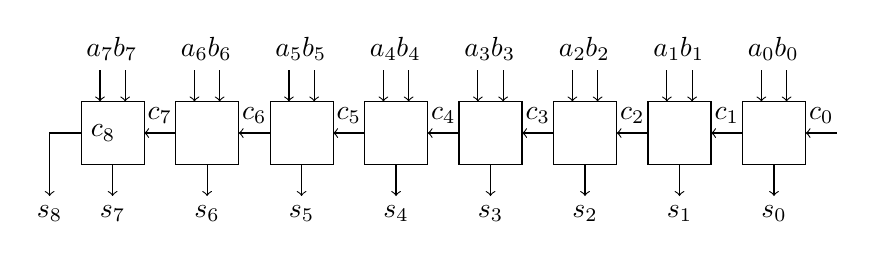
\begin{tikzpicture}[scale=0.4]
    \foreach \x [evaluate={\y=int(7-\x);\z=int(8-\x)}] in {0,1,...,7}
    {
        \draw (3*\x,0) rectangle (3*\x+2,2);
        \draw[->] (3*\x+1,0)  -- (3*\x+1,-1) node[anchor=north] {$s_\y$};
        \draw[->] (3*\x+3,1) -- node[midway,anchor=south] {$c_\y$} (3*\x+2,1);
        \draw[->] (3*\x+0.6,3) node[anchor=south] {$a_\y$} -- (3*\x+0.6,2) ;
        \draw[->] (3*\x+1.4,3) node[anchor=south] {$b_\y$} -- (3*\x+1.4,2) ;
    }
    \draw[->] (0,1) node[anchor=west] {$c_8$} -- (-1,1) -- (-1,-1) node[anchor=north] {$s_8$};
\end{tikzpicture}
}
\caption{}
\end{figure}

全加器接收三个输入$a,b,c_i$,其中$a,b$分别是两个加数,$c_i$是输入进位。全加器产生两个输出$s,c_o$,其中$s$是和,$c_o$是输出进位。全加器的真值表如\autoref{tab1819}。这个逻辑我们在\autoref{exa3}中已经讨论了。

\begin{table}[!ht]
\centering
\begin{tabular}{ccc|cc}
$a$&$b$&$c_i$&$c_o$&$s$\\\hline
0&0&0&0&0\\
0&0&1&0&1\\
0&1&0&0&1\\
0&1&1&1&0\\
1&0&0&0&1\\
1&0&1&1&0\\
1&1&0&1&0\\
1&1&1&1&1
\end{tabular}
\caption{全加器的真值表}\label{tab1819}
\end{table}

\begin{figure}[!ht]
\centering
\adjincludegraphics{images/408.png}%
\smarthfill{10}%
\adjincludegraphics{images/409.png}
\caption{四位加法器。红线和蓝线分别表示两个加数,绿线为进位,黄线为和,底端绿线为溢出位。上面低位下面高位。}\label{fig37}
\end{figure}

有了全加器,直接把多个全加器首尾相连,就得到了一个加法器(\autoref{fig37})。这个加法器要求两个加数从低位到高位依次延迟一个逻辑帧输入。

\begin{figure}[!ht]
\centering
\adjincludegraphics{images/410.png}%
\smarthfill{6}%
\adjincludegraphics{images/411.png}
\caption{四位累加器。两个加数依次输入红蓝线。上面低位下面高位。}\label{fig38}
\end{figure}

除了用组合逻辑,我们还可以用时序逻辑做加法器。降频电路有逢二进一的特性,所以可以直接用降频电路做一个加法器(\autoref{fig38})。与组合逻辑加法器不同,时序逻辑加法器实质上是累加器,如果不复位,那么每次输入都会直接累加到上一次的结果上。在时序逻辑加法器中,第二个加数各位要在同一个逻辑帧输入,或者低位延迟输入,这与组合逻辑加法器恰好相反。

在加法器上,时序逻辑的另一个优点是,把降频电路改成递次电路,就可以直接做任何进制的累加。\bilibili{av40474377/}中的进制转换实际上就是做了一个十进制累加器,每修改一个二进制数位就向累加器中加一个值或减一个值。

\subsection{减法器(Subtractor)}
有了补码这个工具,减法器和加法器就可以共用一个电路,我们只需要增加一些部件将其中一个加数取反加一。取反的操作是容易的,而加一的操作正好可以借用\autoref{tab1406}中我们没有用到的$c_0$。做出的组合逻辑加减法器如\autoref{fig39}所示,需要注意的是加法器的输入从低位到高位延迟一个逻辑帧,所以对每个数位取反的时候也要从低位到高位延迟一个逻辑帧,完成这项工作的是\autoref{fig39}中最右边一列逻辑门。

\begin{figure}[!ht]
\centering
\adjincludegraphics{images/412.png}%
\smarthfill{10}%
\adjincludegraphics{images/413.png}
\caption{四位加减法器。顶端黄线控制加减法,0为加法,1为减法。计算加法时红线和蓝线分别表示两个加数。计算减法时蓝线为被减数,红线为减数。黄线为和,底端绿线为溢出位。上面低位下面高位。}\label{fig39}
\end{figure}

时序逻辑的减法器同样是使用补码运算,这里不给出具体实现。

\subsection{比较器(Comparator)}
比较两个数的大小,最简单的就是从高位向低位逐位比较。例如比较$a_{[7:0]}$和$b_{[7:0]}$两个8位二进制数,首先比较最高位$a_7$和$b_7$,如果它们相等再比较$a_6$和$b_6$,依此类推。最后我们可以得到一个逻辑表达式:
\[\begin{split}
a_{[7:0]}\mathtt{>}b_{[7:0]}=&(a_7\mathtt{>}b_7)(a_7\mathtt{==}b_7\& a_6\mathtt{>}b_6)(a_7\mathtt{==}b_7\& a_6\mathtt{==}b_6\& a_5\mathtt{>}b_5)\\
&(a_7\mathtt{==}b_7\& a_6\mathtt{==}b_6\& a_5\mathtt{==}b_5\& a_4\mathtt{>}b_4)\\
&(a_7\mathtt{==}b_7\& a_6\mathtt{==}b_6\& a_5\mathtt{==}b_5\& a_4\mathtt{==}b_4\& a_3\mathtt{>}b_3)\\
&(a_7\mathtt{==}b_7\& a_6\mathtt{==}b_6\& a_5\mathtt{==}b_5\& a_4\mathtt{==}b_4\& a_3\mathtt{==}b_3\& a_2\mathtt{>}b_2)\\
&(a_7\mathtt{==}b_7\& a_6\mathtt{==}b_6\& a_5\mathtt{==}b_5\& a_4\mathtt{==}b_4\& a_3\mathtt{==}b_3\& a_2\mathtt{==}b_2\& a_1\mathtt{>}b_1)\\
&(a_7\mathtt{==}b_7\& a_6\mathtt{==}b_6\& a_5\mathtt{==}b_5\& a_4\mathtt{==}b_4\& a_3\mathtt{==}b_3\& a_2\mathtt{==}b_2\& a_1\mathtt{==}b_1\& a_0\mathtt{>}b_0)
\end{split}\]
用\autoref{sec23}中的导出公式,我们得到了只包含初等布尔运算的逻辑表达式:
\[\begin{split}
a_{[7:0]}>b_{[7:0]}=&(a_7\&\textrm{\~{}}b_7)(\textrm{\~{}}a_7b_7\& a_6\&\textrm{\~{}}b_6)(\textrm{\~{}}a_7b_7\&\textrm{\~{}}a_6b_6\& a_5\&\textrm{\~{}}b_5)\\
					&(\textrm{\~{}}a_7b_7\&\textrm{\~{}}a_6b_6\&\textrm{\~{}}a_5b_5\& a_4\&\textrm{\~{}}b_4)\\
					&(\textrm{\~{}}a_7b_7\&\textrm{\~{}}a_6b_6\&\textrm{\~{}}a_5b_5\&\textrm{\~{}}a_4b_4\& a_3\&\textrm{\~{}}b_3)\\
					&(\textrm{\~{}}a_7b_7\&\textrm{\~{}}a_6b_6\&\textrm{\~{}}a_5b_5\&\textrm{\~{}}a_4b_4\&\textrm{\~{}}a_3b_3\& a_2\&\textrm{\~{}}b_2)\\
					&(\textrm{\~{}}a_7b_7\&\textrm{\~{}}a_6b_6\&\textrm{\~{}}a_5b_5\&\textrm{\~{}}a_4b_4\&\textrm{\~{}}a_3b_3\&\textrm{\~{}}a_2b_2\& a_1\&\textrm{\~{}}b_1)\\
					&(\textrm{\~{}}a_7b_7\&\textrm{\~{}}a_6b_6\&\textrm{\~{}}a_5b_5\&\textrm{\~{}}a_4b_4\&\textrm{\~{}}a_3b_3\&\textrm{\~{}}a_2b_2\&\textrm{\~{}}a_1b_1\& a_0\&\textrm{\~{}}b_0)
\end{split}\]

\begin{figure}
\centering
\adjincludegraphics{images/396.png}%
\smarthfill{22}%
\adjincludegraphics{images/397.png}
\caption{逐位比较器。上方火把表示$b_{[7:0]}$,左边高位右边低位;右侧火把表示$a_{[7:0]}$,下方高位上方低位;左下火把表示$a_{[7:0]}\mathtt{>}b_{[7:0]}$。}\label{fig33}
\end{figure}
将这个逻辑表达式转换为电路如\autoref{fig33}所示。

比较两个数的大小,除了逐位比较之外,还可以直接将两个数做减法,并判断结果的正负性。减法器我们已经做过了,而补码表示中,一个数的正负可以直接通过最高位得出。这里有两个细节的问题。无符号整数没有符号位,如何比较两个无符号整数的大小?有符号整数的两数之差可以达到$127-(-128)=255=11111111$,而这个数作为有符号整数实际上表示$-1$,即小于0。如何处理这些特殊情况?事实上我们这里的比较器只能比较无符号整数,而所谓的“最高位”实际上指的是\autoref{tab1406}中的溢出位$s_8$。对于有符号整数有两种处理方法:第一种是首先判断符号,如果符号相等,再做无符号整数的比较;第二种是把两个数都加$128$,这样就把$-128\sim127$的范围变成了$0\sim255$,然后做无符号整数的比较即可。

比较两个数是否相等,也有两种解法,一种是直接逐位比较,另一种是判断它们的差是否为0。这两种方法并没有绝对的优劣,虽然逐位比较的电路会比较简单,但是判断差值的电路可以直接附加在其他功能上,例如加法器。

\subsection{乘法器(Multiplier)}
乘法是加法的推广,乘法器也是加法器的推广。我们首先来看二进制乘法的竖式计算。因为乘法规模较大,这里给出4位乘法的例子(\autoref{tab6585})。

\begin{figure}[!ht]
$$
\begin{array}{ccccccccc}
&&&&a_3&a_2&a_1&a_0\\
&&&&b_3&b_2&b_1&b_0\\\hline
&&&&b_0\&a_3&b_0\&a_2&b_0\&a_1&b_0\&a_0\\
&&&b_1\&a_3&b_1\&a_2&b_1\&a_1&b_1\&a_0\\
&&b_2\&a_3&b_2\&a_2&b_2\&a_1&b_2\&a_0\\
&b_3\&a_3&b_3\&a_2&b_3\&a_1&b_3\&a_0\\\hline
H_3&H_2&H_1&H_0&l_3&l_2&l_1&l_0
\end{array}
$$
\caption{乘法竖式计算}\label{tab6585}
\end{figure}

从\autoref{tab6585}可以看出来,做一个4位乘法实际上就是做4个数的加法。4个数的加法,可以按照运算顺序拆分成三次2个数的加法,如\autoref{fig79}所示。

\begin{figure}[!ht]
\centering
\begin{tikzpicture}
    \draw (0,0) rectangle node{加法器} (5,1);
    \draw (0,2) rectangle node{加法器} (5,3);
    \draw (0,4) rectangle node{加法器} (5,5);
    
    \draw[->] (2,6) node[anchor=south]{$a_1$} -- (2,5);
    \draw[->] (3,6) node[anchor=south]{$a_2$} -- (3,5);
    \draw[->] (2,4)  -- node[midway,anchor=east]{$a_1+a_2$} (2,3);
    \draw[->] (6,3.5) node[anchor=west]{$a_3$} -- (3,3.5) -- (3,3);
    \draw[->] (2,2)  -- node[midway,anchor=east]{$a_1+a_2+a_3$} (2,1);
    \draw[->] (6,1.5) node[anchor=west]{$a_4$} -- (3,1.5) -- (3,1);
    \draw[->] (2.5,0) -- (2.5,-1) node[anchor=north]{$a_1+a_2+a_3+a_4$};
\end{tikzpicture}
\caption{四个加数$a_1,a_2,a_3,a_4$连加}\label{fig79}
\end{figure}

把\autoref{fig79}中的加法器展开成串联的全加器,就得到了四位乘法器的结构示意图(\autoref{fig80})。

\begin{figure}[!ht]
\centering
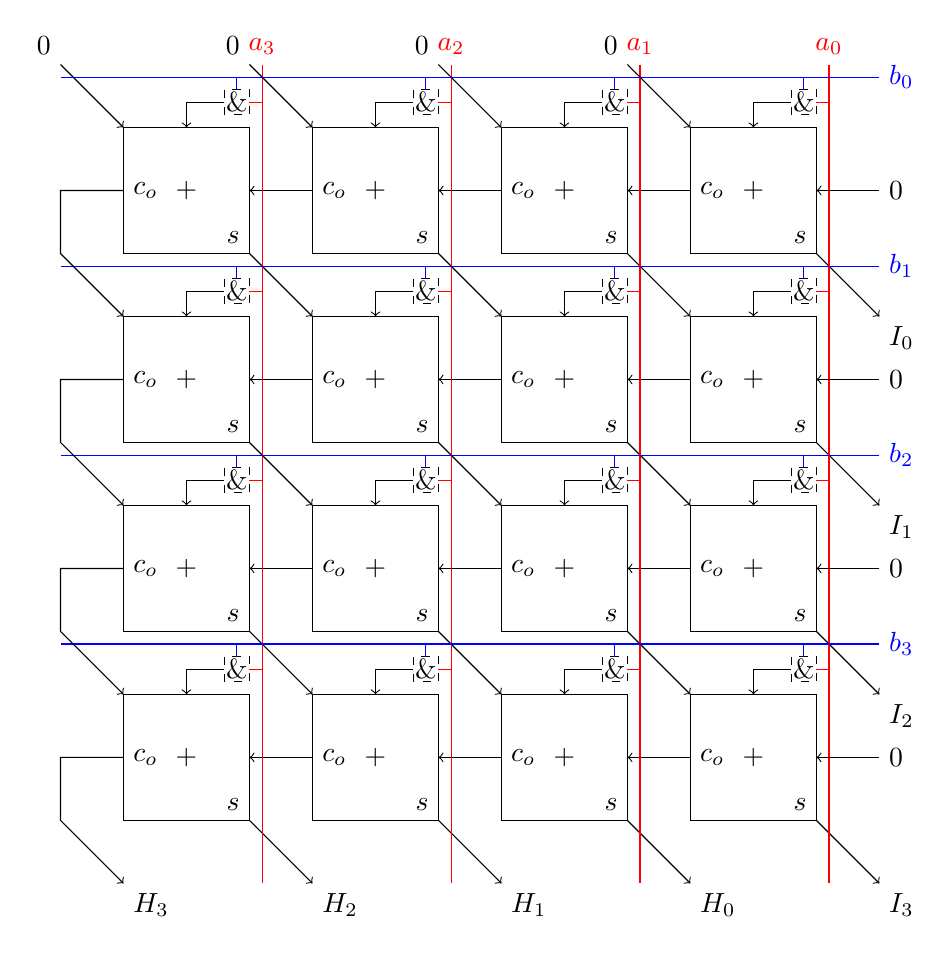
\begin{tikzpicture}[scale=0.8]
    \foreach \x [evaluate={\z=int(3-\x)}] in {0,1,2,3}
        \foreach \y [evaluate={\w=int(3-\y)}] in {0,1,2,3} {
            \draw (3*\x,3*\y) rectangle node {$+$} (3*\x+2,3*\y+2); % 全加器框架
            \draw[dashed] (3*\x+1.6,3*\y+2.2) rectangle node {\&} (3*\x+2,3*\y+2.6);
            \draw[->] (3*\x+1.6,3*\y+2.4) -- (3*\x+1,3*\y+2.4) -- (3*\x+1,3*\y+2);
            \draw[blue] (3*\x+1.8,3*\y+2.6) -- (3*\x+1.8,3*\y+2.8);
            \draw[red] (3*\x+2,3*\y+2.4) -- (3*\x+2.2,3*\y+2.4);
            \draw[->] (3*\x+2,3*\y) node[anchor=south east] {$s$} -- (3*\x+3,3*\y-1); % 和输出
        }
    \foreach \x in {1,2,3}
        \foreach \y in {0,1,2,3}
            \draw[->] (3*\x,3*\y+1) node[anchor=west] {$c_o$} -- (3*\x-1,3*\y+1); % 进位连接
    \foreach \x [evaluate={\z=int(3-\x)}] in {0,1,2,3}{
        \draw[->,] (3*\x-1,12) node[anchor=south east] {$0$} -- (3*\x,11); % 第一排缺省加数
        \draw (3*\x,-1) node[anchor=north west] {$H_\z$}; % 结果高四位
        \draw[red] (3*\x+2.2,12) node[anchor=south] {$a_\z$} -- (3*\x+2.2,-1); %乘数1输入
    }
    \foreach \y [evaluate={\w=int(3-\y)}] in {0,1,2,3}{
        \draw (12,3*\y-1) node[anchor=north west] {$I_\w$}; % 结果低四位
        \draw[->] (0,3*\y+1) node[anchor=west] {$c_o$} -- (-1,3*\y+1) -- (-1,3*\y) -- (0,3*\y-1); % 左边一列进位输出
        \draw[->] (12,3*\y+1) node[anchor=west] {$0$} -- (11,3*\y+1); % 右边一列进位输入
        \draw[blue] (12,3*\y+2.8) node[anchor=west] {$b_\w$}-- (-1,3*\y+2.8); % 乘数2输入
    }
\end{tikzpicture}
\caption{四位乘法器结构示意图。大的实线方框表示全加器,$c_o$表示进位输出,$s$表示和输出。小的虚线方框表示与门,红蓝线输入,黑线输出。两个乘数分别从上方和右方输入,乘积的低位从右边输出,高位从下边输出。全加器缺少的输入补零。左右相邻的两个全加器,右边的早一个逻辑帧;上下相邻的两个全加器,上边的早两个逻辑帧。}\label{fig80}
\end{figure}

乘法器的单个单元电路见\autoref{fig81},其中用不同颜色的背景墙标记区域和线路。橙色区域为全加器。黄色区域是与门。蓝色线路是从右边输入的乘数,每经过一个单元要延迟1个逻辑帧。红色线路是从上边输入的乘数,每经过一个单元要延迟2个逻辑帧。紫色线路是横向的进位传递。绿色线路是从左上到右下的和传递。

\begin{figure}[!ht]
\centering
\adjincludegraphics{images/436.png}
\caption{乘法器单个单元的结构}\label{fig81}
\end{figure}

单元堆叠后的效果见\autoref{fig82},其中每个单元大小3*7。优化过程用到了如下的接线技巧:
\begin{itemize}
	\item 左右方向上红蓝线循环,便于接线。
	\item 相邻两列错位,便于进位和横向乘数的传递。
	\item 纵向的逻辑延迟用到了一个异或门,从而这个门不需要为经过的绿线让路。
	\item 与门利用了等式$a\&b=\textrm{\~{}} ab\&b$,便于接线。
\end{itemize}

\begin{figure}[!ht]
\centering
\adjincludegraphics{images/437.png}
\caption{堆叠优化后的效果}\label{fig82}
\end{figure}

\subsection{除法器(Divider)}
1
\subsection{移位器(Shifter)}
移位又分为逻辑移位、算术移位、循环移位,其中逻辑移位和算术移位应用较广。

\begin{figure}[!ht]
\centering
\subfloat[]{\label{i414}\adjincludegraphics{images/414.png}}%
\smarthfill{25}[3]%
\subfloat[]{\label{i415}\adjincludegraphics{images/415.png}}%
\smarthfill{25}[3]%
\subfloat[]{\label{i416}\adjincludegraphics{images/416.png}}
\caption{递次电路移位。\protect\subref{i414}逻辑右移一位;\protect\subref{i415}算术右移一位;\protect\subref{i416}循环右移一位。}\label{fig40}
\end{figure}

如果只移一位的话,这三种移位都可以通过递次电路实现,如\autoref{fig40}所示。

\begin{figure}[p]
\centering
\subfloat[逻辑右移]{
	\adjincludegraphics{images/400.png}%
	\smarthfill{38}%
	\adjincludegraphics{images/401.png}
}

\subfloat[算术右移]{
	\adjincludegraphics{images/402.png}%
	\smarthfill{38}%
	\adjincludegraphics{images/403.png}
}

\subfloat[经过简单优化的算术右移]{
	\adjincludegraphics{images/404.png}%
	\smarthfill{38}%
	\adjincludegraphics{images/405.png}
}
\caption{组合逻辑原理的移位器。右侧三个火把从上到下作用依次为移1位、移2位、移4位。}\label{fig35}
\end{figure}

如果要移任意位,递次电路大概率会爆门,此时需要考虑其他方案。一个简单的思路是使用\autoref{fig35}所示的组合逻辑。这个组合逻辑的缺点是,被移位数的所有数位输入要在同一个逻辑帧,而移位量的数位要在各个逻辑帧依次输入,调节逻辑同步较复杂。此外,由于逻辑门的取向问题,这种方法不适用于循环移位。

\begin{figure}[!ht]
\centering
\adjincludegraphics{images/417.png}%
\smarthfill{64}%
\adjincludegraphics{images/418.png}
\caption{移位器。纵向的红蓝线输入待移位的数。横向红蓝线输入移位的位数。通过顶端的逻辑灯激活对应的输出。底端绿线用于切换逻辑移位和算术移位。}\label{fig41}
\end{figure}

事实上,因为数字电路结构都相对复杂,在泰拉瑞亚中想做一定规模的数字电路,一定要考虑利用\nameref{sec17}技术传输数据。\nameref{sec17}技术通过在不同逻辑帧发送不同数位传播数据,我们可以通过这一特点设计专门兼容\nameref{sec17}的移位器。\autoref{fig41}通过选取网线输出的起始数位实现移位功能。

\subsection{随机数生成器(Random Number Generator)}
在现实中需要用复杂算法实现的功能,在泰拉瑞亚中反而异常简单。直接使用8个1/2概率的故障逻辑门,我们就可以随机生成8位二进制数。
\vspace{5cm}

没了。

\subsection{进制转换}

\paragraph*{方法一} 直接用定义式$a_{n:0}=a_n2^n+a_{n-1}2^{n-1}+\cdots+a_02^0$。要利用这个式子将二进制转换为十进制,需要做一个十进制加法器,然后存储2的各次幂的十进制值。\bilibili{av40474377}就是用的这种方法。

十进制转二进制可以用同样的原理,做一个二进制加法器,然后存储10的各次幂的二进制值。

\paragraph*{方法二} 利用\autoref{sec30}和\autoref{sec31}介绍的方法。在竖式的每一步中,我们需要做一个查表的操作,然后错一位。这个查表的操作实际上是一个组合逻辑,如\autoref{tab12}所示。

\begin{table}[!ht]
\centering
\begin{tabular}{|c|c|}
\hline
二进制&BCD\\\hline
0000&0000\\\hline
0001&0001\\\hline
0010&0010\\\hline
0011&0011\\\hline
0100&0100\\\hline
0101&1000\\\hline
0110&1001\\\hline
0111&1010\\\hline
1000&1011\\\hline
1001&1100\\\hline
\end{tabular}
\caption{二进制转BCD则从左到右查,BCD转二进制则从右到左查。}\label{tab12}
\end{table}

二进制转BCD和BCD转二进制对应不同的真值表,我们需要分开设计。

\section{存储电路}
一个存储电路总是要有一个用于存放数据的阵列和一个选择数据的\termMUX 。

\subsection{\termMUX (Multiplexer, MUX)}
\emph{\termMUX}又名\emph{数据选择器}(Data Selector)。\termMUX 接收一个二进制地址,激活该地址代表的位置。一个经典的四位\termMUX 如\autoref{fig42}所示。

\begin{figure}[!ht]
\centering
\adjincludegraphics{images/419.png}%
\smarthfill{36}%
\adjincludegraphics{images/420.png}
\caption{经典四位\termMUX。红蓝线表示地址,上面高位下面低位。绿线双激活输出。16个逻辑门从左到右依次表示0000到1111。}\label{fig42}
\end{figure}

我们在\nameref{sec2:2}中曾见过相似的电路,事实上那个就是状态版的\termMUX 。本小节中我们通过\nameref{sec33}实现了激活版的\termMUX 。

\subsection{只读存储器(Read-Only Memory)}
只读存储器用于存储事先设计好的、固定的数据。这些数据不需要在使用时修改,所以一般是通过物理方式直接做在电路中。
\begin{figure}[!ht]
    \centering
	\subfloat[横向输入纵向输出]{\label{fig49}\adjincludegraphics{images/342.png}\adjincludegraphics{images/341.png}}
	
	\subfloat[纵向输入横向输出]{\label{fig50}\adjincludegraphics{images/343.png}\adjincludegraphics{images/344.png}}%
    \smarthfill{50}%
	\subfloat[纵向输入横向输出]{\label{fig51}\adjincludegraphics{images/346.png}\adjincludegraphics{images/345.png}}
    \caption{ROM的三种设计。}\label{fig48}
\end{figure}
\autoref{fig48}展示了三种ROM设计。\autoref{fig49}使用故障逻辑灯存储数据。一根横线激活时,只有经过的故障逻辑灯下方的逻辑门才会激活。因为存储器要与\termMUX 配合,而\termMUX 是纵向输出,所以\autoref{fig49}目前没有实用价值。\autoref{fig50}和\autoref{fig51}都是通过接线存储数据,也是有广泛应用的两种ROM。两个电路在实现方式上的区别是,\autoref{fig50}通过连接输出线与逻辑门来存储,而\autoref{fig51}通过连接输入线与逻辑灯来存储。占用空间方面,\autoref{fig50}占用高度较低(1.5格/bit),\autoref{fig51}占用高度较高(2格/bit)。逻辑同步方面,\autoref{fig51}的输出是同步的,而\autoref{fig50}不同步,在本来就需要不同步的场景(例如很多\nameref{sec34}和\nameref{sec17}),\autoref{fig50}更好。

\nameref{sec2:2}中,\autoref{i36:37}就是状态式的\termMUX ,\autoref{i42:43}的下半部分电路就是\autoref{fig50}样式的ROM。只有有限个输出情况的显示器都可以通过ROM实现。

\subsection{只写存储器(Write-Only Memory)}
1
\subsection{随机存储器(Random Access Memory)}
1
\subsection{寄存器(Register)}
1
\subsection{栈(Stack)}
1

\section{分段显示器化简理论}
1
\subsection{分段显示器主要结构}
1
\subsection{显示矩阵、分段矩阵和数字矩阵}
1
\subsection{矩阵的初等变换}
1
\subsection{化简原理与细节}
1

\section{处理器结构}
1
\subsection{汇编语言}
1
\subsection{机器语言}
1
\subsection{处理器的拓扑结构}
1
\subsection{数据路径(Data Path)}
1
\include{chapters/Sources}
%\include{chapters/chapter8}
\chapter{更多电路专题}

在前面我们已经学习了所有电路原理。在这一章中我们以电路功能分类,介绍一些常用的电路模块。

\section{递次电路}\label{sec2}
在\autoref{sec35}中我们介绍了传统递次电路的原理,这里我们来看一下各式各样的递次电路。

\subsection{传统递次电路}
“传统”递次电路即为在多个故障逻辑门中简单循环的电路。我们在后面的推广递次和多级递次中可以看到递次电路的其他思路。

\begin{figure}[!ht]
    \centering
	\subfloat[传统递次]{
		\label{fig52}
		\adjincludegraphics{images/72.png}%
		\quad%
		\adjincludegraphics{images/73.png}
	}
	
	\subfloat[带复位的传统递次]{
		\label{fig53}
		\adjincludegraphics{images/106.png}%
		\quad%
		\adjincludegraphics{images/107.png}
	}%
	\smarthfill{44}%
    \subfloat[斜式传统递次]{
		\label{fig54}
		\adjincludegraphics{images/78.png}%
		\quad%
		\adjincludegraphics{images/79.png}
	}
	\subfloat[密排传统递次]{
		\label{fig55}
		\adjincludegraphics{images/82.png}%
		\quad%
		\adjincludegraphics{images/83.png}
	}
	\subfloat[密排带复位传统递次]{
		\label{fig56}
		\adjincludegraphics{images/317.png}%
		\quad%
		\adjincludegraphics{images/318.png}
	}
	\caption{常用的传统递次电路}
\end{figure}

\autoref{fig52}和\autoref{fig53}就是我们在\autoref{sec35}中已经学习的基础电路。\autoref{fig53}是我们在\autoref{sec36}中使用到的模块。\autoref{fig55}耗尽了电线颜色,所以实际应用时需要谨慎选择。

\autoref{fig56}的复位部分使用了\nameref{sec37}。

\subsection{传统双向递次电路}\label{sec3}
双向递次电路就是可以正反两个方向循环的递次电路。正反分别用两根线控制。

\begin{figure}[!ht]
    \centering
    \subfloat[传统双向递次]{
		\adjincludegraphics{images/263.png}%
		\quad%
		\adjincludegraphics{images/264.png}
	}%
	\smarthfill{42}%
    \subfloat[密排传统双向递次]{
		\adjincludegraphics{images/261.png}%
		\quad%
		\adjincludegraphics{images/262.png}
	}
	
    \subfloat[带复位的传统双向递次]{
		\adjincludegraphics{images/265.png}
		\quad
		\adjincludegraphics{images/266.png}
	}
	\caption{传统双向递次电路}
\end{figure}

\subsection{推广递次电路}
递次电路能形成循环,是靠的故障逻辑门改变逻辑灯状态,而逻辑灯状态又能反过来决定故障逻辑门是否激活。换言之,每一步中电路的状态都可以决定下一步的状态。这样依次下去,就形成了一个状态链。我们有理由相信,在某些特定的接线方式下,状态链会形成循环。

\begin{example}{}{}
分析如\autoref{fig59}所示的4-传统递次电路。
\begin{figure}[H]
\centering
\adjincludegraphics{images/416.png}
\caption{}\label{fig59}
\end{figure}
\begin{proof}[解]
4-传统递次总共有16种状态,它们对应的后继如\autoref{tab14}所示。
\begin{table}[H]
\centering
\begin{tabular}{|c|c|}
\hline
当前状态&下一状态\\\hline
0000&0000\\\hline
0001&1000\\\hline
0010&0001\\\hline
0011&1001\\\hline
0100&0010\\\hline
0101&1010\\\hline
0110&0011\\\hline
0111&1011\\\hline
1000&0100\\\hline
1001&1100\\\hline
1010&0101\\\hline
1011&1101\\\hline
1100&0110\\\hline
1101&1110\\\hline
1110&0111\\\hline
1111&1111\\\hline
\end{tabular}
\caption{}\label{tab14}
\end{table}

根据\autoref{tab14},我们得出4-传统递次的所有循环:
\begin{align*}
0000&\to 0000\\
1000&\to 0100\to 0010\to 0001\to 1000\\
0110&\to 0011\to 1001\to 1100\to 0110\\
0101&\to 1010\to 0101\\
0111&\to 1011\to 1101\to 1110\to 0111\\
1111&\to 1111
\end{align*}
4-传统递次一共有6个循环,其中2个1循环、1个2循环、3个4循环。
\end{proof}
\end{example}


\begin{example}{}{}
分析如\autoref{fig57}所示的推广递次电路。
\begin{figure}[H]
\centering
\adjincludegraphics{images/426.png}
\caption{}\label{fig57}
\end{figure}
\begin{proof}[解]
\begin{table}[H]
\centering
\begin{tabular}{|c|c|}
\hline
当前状态&下一状态\\\hline
0000&0000\\\hline
0001&1000\\\hline
0010&0001\\\hline
0011&1001\\\hline
0100&0010\\\hline
0101&1010\\\hline
0110&0011\\\hline
0111&1011\\\hline
1000&0110\\\hline
1001&1110\\\hline
1010&0111\\\hline
1011&1111\\\hline
1100&0100\\\hline
1101&1100\\\hline
1110&0101\\\hline
1111&1101\\\hline
\end{tabular}
\caption{}\label{tab15}
\end{table}
根据\autoref{tab15},我们得出该推广递次的所有循环:
\begin{align*}
0000\to &0000\\
0001\to &1000\to 0110\to 0011\to 1001\to 1110\to 0101\to 1010\to \\
        &0111\to 1011\to 1111\to 1101\to 1100\to 0100\to 0010\to 0001
\end{align*}
该推广递次一共有2个循环,其中1个1循环、1个15循环。
\end{proof}
\end{example}


不难看出,无论推广递次如何连接,$0000\to 0000$的1循环是不会变的,我们把这个循环叫做\textbf{平凡循环}并在之后的讨论中忽略它。如果一个推广递次的所有非零状态共同构成了一个循环,那么我们把这个循环叫做\textbf{全循环}。推广递次连接的多样化、状态的多样化、循环的多样化带来了更多的可能性。

\begin{example}{}{}
分析\autoref{fig58}中的降频电路。
\begin{figure}[H]
\centering
\adjincludegraphics{images/332.png}
\caption{}\label{fig58}
\end{figure}
\begin{proof}[解]
该电路分为两部分:左边两个门为2-推广递次电路,右边一个门为2-降频电路,2-推广递次的绿线接到2-降频电路的输入。

分析推广递次的输出时,不光要分析各个灯的状态,还要分析各根线的状态。本例中2-推广递次的两个灯与两根线的状态如\autoref{tab16}所示,其中两根线的初始状态设为0。

\begin{table}[H]
\centering
\begin{tabular}{|c|c|c|c|}
\hline
状态编号&两灯状态&蓝线状态&绿线状态\\\hline
0&10&0&0\\\hline
1&01&1&0\\\hline
2&11&0&1\\\hline
\end{tabular}
\caption{}\label{tab16}
\end{table}

这个推广递次的循环为3,而且每个循环中绿线激活两次,通过2-降频电路后,每个循环中火把被激活一次。所以\autoref{fig58}中的降频电路是3-降频电路。

如果使用3-传统递次电路实现降频,因为摆线的原因,电路的宽或高至少要增加一格。推广递次在这种简单功能上有体积的优势。

如果去掉最右边的2-降频电路,左边的2-推广递次就会变成一个不均匀降频电路,或者说,(1,2)-降频电路,即周期在1与2切换。改变推广递次的门数与接线就可以得到各种各样的不均匀降频电路。串联不均匀降频电路可以得到输出更复杂的不均匀降频电路,例如串联两个(1,2)-降频电路,可以得到(1,3,2,3)-降频电路,其推导过程留给读者。

\end{proof}
\end{example}


并非所有推广递次都可以产生非平凡循环。

\begin{example}{}{}
\autoref{fig60}所示推广递次的状态链见\autoref{fig61}。这个状态链是一棵树,不包含任何一个非平凡循环。
\begin{figure}[H]
\centering
\adjincludegraphics{images/414.png}
\caption{}\label{fig60}
\end{figure}
\begin{figure}[H]
\centering
\begin{forest} for tree={edge={<-},grow=west},
	[0000,name=s
		[0001
			[0010
				[0100
					[1000]
					[1001]]
				[0101
					[1010]
					[1011]]]
			[0011
				[0110
					[1100]
					[1101]]
				[0111
					[1110]
					[1111]]]]]
	\draw[->] (s) to[out=45,in=-45,looseness=3] (s);
\end{forest}
\caption{}\label{fig61}
\end{figure}
\end{example}

\begin{example}{}{}
\autoref{fig62}所示推广递次的状态链见\autoref{fig63}。这个状态链由两棵树组成。
\begin{figure}[H]
\centering
\adjincludegraphics{images/415.png}
\caption{}\label{fig62}
\end{figure}
\begin{figure}[H]
\centering
\begin{forest} for tree={edge={<-},grow=west},
	[0000,name=s
		[0001
			[0010
				[0100]
				[0101]]
			[0011
				[0110]
				[0111]]]]
	\draw[->] (s) to[out=45,in=-45,looseness=3] (s);
\end{forest}
\quad
\begin{forest} for tree={edge={<-},grow=east},
	[1111,name=s
		[1110
			[1101
				[1011]
				[1010]]
			[1100
				[1001]
				[1000]]]]
	\draw[->] (s) to[out=135,in=-135,looseness=3] (s);
\end{forest}
\caption{}\label{fig63}
\end{figure}

\end{example}

\begin{example}{}{}
\autoref{fig65}所示推广递次的状态链见\autoref{fig64},其中既有环结构也有树结构。
\begin{figure}[H]
\centering
\adjincludegraphics{images/427.png}
\caption{}\label{fig65}
\end{figure}
\begin{figure}[H]
\centering
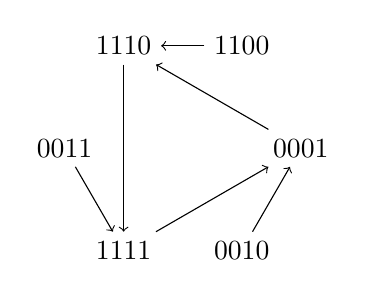
\begin{tikzpicture}
\newdimen\R
\R=1.5cm;
\node (s1) at (0:\R) {0001};
\node (se) at (120:\R) {1110};
\node (sf) at (240:\R) {1111};
\node (s2) at (300:\R) {0010};
\node (s3) at (180:\R) {0011};
\node (sc) at (60:\R) {1100};
\path [->]
    (s1) edge (se)
    (se) edge (sf)
    (sf) edge (s1)
    (s2) edge (s1)
    (s3) edge (sf)
    (sc) edge (se);
\end{tikzpicture}
\quad
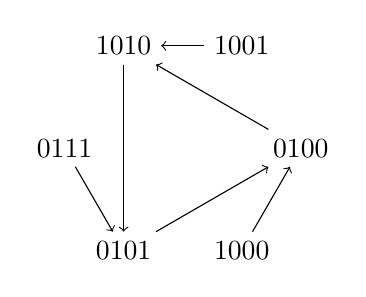
\begin{tikzpicture}
\newdimen\R
\R=1.5cm;
\node (s1) at (0:\R) {0100};
\node (se) at (120:\R) {1010};
\node (sf) at (240:\R) {0101};
\node (s2) at (300:\R) {1000};
\node (s3) at (180:\R) {0111};
\node (sc) at (60:\R) {1001};
\path [->]
    (s1) edge (se)
    (se) edge (sf)
    (sf) edge (s1)
    (s2) edge (s1)
    (s3) edge (sf)
    (sc) edge (se);
\end{tikzpicture}
\quad
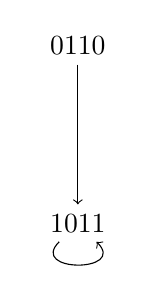
\begin{tikzpicture}
\newdimen\R
\R=1.3cm;
\node (se) at (120:\R) {0110};
\node (sf) at (240:\R) {1011};
\path [->] (se) edge (sf);
\draw [->] (sf) to[out=-135,in=-45,looseness=3] (sf);
\end{tikzpicture}
\quad
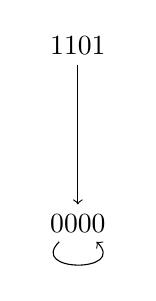
\begin{tikzpicture}
\newdimen\R
\R=1.3cm;
\node (se) at (120:\R) {1101};
\node (sf) at (240:\R) {0000};
\path [->] (se) edge (sf);
\draw [->] (sf) to[out=-135,in=-45,looseness=3] (sf);
\end{tikzpicture}
\caption{}\label{fig64}
\end{figure}
\end{example}

目前除了暴力穷举之外尚无法预测推广递次的行为,设计推广递次靠尝试与经验。

\section{驱动}

\subsection{自定义半砖驱动}
使用假人驱动可以得到60Hz的驱动。如果要进行降频,除了使用降频技术以外,还可以修改半砖装置(\autoref{i235:236})。

\begin{figure}[!ht]
\begin{center}
\subfloat[]{
\label{i235}
\adjincludegraphics{images/235.png}
}%
\smarthfill{21}%
\subfloat[]{
\label{i236}
\adjincludegraphics{images/236.png}
}
\end{center}
\caption{\protect\subref{i235}只使用一个压力板,频率降为30Hz;\protect\subref{i235}加长半砖,频率降为20Hz。}
\label{i235:236}
\end{figure}

\subsection{其他驱动摘要}
由于使用计时器和假人驱动已经可以随意控制时间,其他驱动也就逐步淡出。但是为了保留思路,仍介绍这些驱动,说不定什么时候有奇效。
\begin{itemize}
\item 生物驱动:利用生物行走速度固定构造的驱动。往往利用雕像刷怪。与玩家距离不能太远,否则生物会消失。雕像怪物速度测试\bilibili{av22739934}。在1.3.0.1版本引入傀儡之前,半砖驱动一般使用骷髅雕像生成的骷髅。
\item 柱形驱动:利用下层叠平台的稳定间隔构造的驱动。链接\bilibili{av23028215}。
\item 传送带驱动:已介绍。虽然仍为满频驱动,但是需要限制玩家自由。
\item 机关驱动:利用各种可以发射射弹的电路物品与青绿压力垫板构造的驱动。由于射弹速度各不相同,并且还受液体减速影响,控制不如假人驱动简单。但是由于占用空间可以很小,该类驱动仍有一定价值。
\item 传送机驱动:利用传送机传送对象相对于传送区域位置不变的特性。见\autoref{i219:220}

\begin{figure}[!ht]
\begin{center}
\subfloat[]{
\label{i219}
\adjincludegraphics{images/219.png}
}%
\smarthfill{9}%
\subfloat[]{
\label{i220}
\adjincludegraphics{images/220.png}
}
\end{center}
\caption{\protect\subref{i219}踩踏红压力板时触发传送机,传送后会悬空一格,坠落到压力板上时继续传送,如此循环;\protect\subref{i220}传送后悬空半格。}
\label{i219:220}
\end{figure}

\end{itemize}

\section{传感器}
泰拉瑞亚中已经自带了很多传感器,例如压力板、感应器等。在实际使用中,我们有时需要检测游戏自带传感器检测不了的东西,那么就需要另外设计传感器。

\subsection{开服感应器}
所谓开服感应器,就是在打开地图时激活的电源。只要地图不关闭,该电源就不会再次激活。

最容易想到的就是在重生点放上玩家感应器,并把玩家传送走。但是这样一来,在玩家回程时会再次激活。使用床传送技术\youku{XMTg0NzYxNDg0OA}可以避免这一点,但是无法在退出地图时自动重置。

从打开地图开始,玩家第一次接近傀儡时傀儡影子会在傀儡上生成。傀儡是家具而傀儡影子是敌怪,它们分开结算:家具是固定的,而影子可以移动、受伤害、受debuff。虽然影子不会主动移动,但是会被动移动,例如坠落、传送机传送、半砖传送。当影子受伤害时家具播放动画。影子与家具所在格由于各自的原因均不能摆放前景物块\footnote{前景物块不能摆放在家具图格上或生物碰撞箱上。}。

只要傀儡影子在重生点附近,那么傀儡影子在打开地图时就会重新生成在傀儡上。

最简单的开服感应器如\autoref{i221}。傀儡悬空,下面放有压力板。每次打开地图后傀儡影子生成,掉落在压力板上激活压力板。这个开服感应器略有延迟,延迟长度是傀儡影子掉落到压力板上的时间。一般来说这么短的延迟不会有什么问题。

\begin{figure}[!ht]
\centering
\adjincludegraphics{images/221.png}
\caption{}
\label{i221}
\end{figure}

如果想要更短的延迟,可以考虑在开图瞬间用传送机将傀儡影子传送走,并做一些处理使传送机再次激活时不会将影子传送回(\autoref{i222})。

\begin{figure}[!ht]
\centering
\adjincludegraphics{images/222.png}
\caption{}
\label{i222}
\end{figure}

上面的装置中,传送机激活后1帧,傀儡影子就被半砖推离传送机并触发红压力板,从而不会再传回。但是玩家感应器和测重压力板不会触发传送机,玩家出生在重生点处也不会触发普通压力板。只能用玩家感应器或测重压力板触发机关,然后用青绿压力垫板激活传送机,这样一来在触发机关到青绿压力垫板激活之间又有一个短延迟。

利用液体可以实现无延迟的开服感应器。打开地图的等待界面中有一项是“正在摆放液体”。这一步是将地图中所有不稳定的液体转移到最低处。在\autoref{i11:12}中,刷水机不断地生成水,水进入到左边的细长通道,并被下面的熔岩轨道吸收。当通道足够长并且刷水速度足够快时,通道中始终有水存在。此时退出地图并重新加载地图时,通道中的水被自动放置到最低处的液体感应器上,从而液体感应器激活。其余部分的功能是:将液体感应器上的水排走;打开刷水的1秒计时器。这个装置的触发是没有延迟的,但是会在游戏中一直运行刷水机,可能影响电脑性能。

\subsection{方向感应器}
方向感应器被广泛地使用在电路游戏中,它可以检测到玩家的上下左右移动操作。方向感应器的一种方案如\autoref{i253:254}所示。另一种方案请参考\bilibili{av23633364/?p=7}。

\begin{figure}[!ht]
	\centering
	\adjincludegraphics{images/253.png}%
	\smarthfill{22}%
	\adjincludegraphics{images/254.png}
	\caption{玩家试图左右移动时会触发玩家感应器并实化半砖将玩家推回;试图上平台时平台虚化,玩家掉落;试图下平台时下方半砖实化将玩家推回。}
	\label{i253:254}
\end{figure}

\subsection{刷怪感应器}
刷怪感应器应用于刷怪场和Boss战场中,用来检测各种敌怪生成。大多数敌怪都可以直接触发压力板,所以一般情况下压力板就可以用来做刷怪感应器。穿墙怪不会触发压力板,只能使用特殊方法处理。

一个勉强及格的方案是在玩家周围放置压力板,穿墙怪攻击玩家时,玩家被击退,触发压力板,从而敌怪被检测到。这个方案的缺点是明显的,但是暂时也没有更好的方法。

\section{显示器}
显示器从原理上分为分段显示器、密集矩阵显示器、稀疏矩阵显示器、像素盒显示器。

\subsection{分段显示器}
分段显示器,指根据显示需要,将显示界面分为若干部分分别控制的显示器。在显示器中有部分光源状态始终同步的情况下,将这些光源当作单个光源处理,即为一段。在十进制数显中我们将显示器分为了七段;在二进制数显中分为了两段;在\autoref{dianlujichu}的思考题中,将月相显示器的分段任务留给了读者。

分段之后就可以设计控制电路。\autoref{i42:43}和\autoref{i71}中展示了十进制数显的两种不同控制电路风格。前者逻辑门排列紧密,需要更多排换线器;后者逻辑门有间隔,需要换线器更少但是占用空间更大。由于显示部分本身体积就很小,使用占用空间大的控制电路容易导致接线难看(\autoref{i113:114})。

另外,\autoref{i42:43}和\autoref{i71}展示了十进制数显的两种不同分段方式。一个分段显示器可以有很多种分段方式,不同的分段方式对应不同的控制电路和接线。一个自然的问题是,是否可以设计出一个分段方式使得控制电路最简?答案是,没有一个固定的套路可以使控制电路最简。尽管如此,我们往往还是可以做出部分简化。下面以一个例子来介绍优化分段方式的方法。

我们希望修改十进制数显的分段来减少控制电路的大小。数显初始分段如\autoref{i34:35}所示。在这个分段下,数字与分段的对应关系如\autoref{sjzsxctjxdxsjz}。

\begin{table}[!ht]
\centering
\begin{tabular}{c|ccccccc}
&a&b&c&d&e&f&g\\\hline
0&1&1&1&0&1&1&1\\
1&0&0&1&0&0&1&0\\
2&1&0&1&1&1&0&1\\
3&1&0&1&1&0&1&1\\
4&0&1&1&1&0&1&0\\
5&1&1&0&1&0&1&1\\
6&1&1&0&1&1&1&1\\
7&1&0&1&0&0&1&0\\
8&1&1&1&1&1&1&1\\
9&1&1&1&1&0&1&1
\end{tabular}
\caption{十进制数显传统接线的显示矩阵}\label{sjzsxctjxdxsjz}
\end{table}

上面的矩阵在$\mathbb{F}_2$\footnote{域$\mathbb{F}_2$包含0,1两个元素,可以将0看作偶数,1看作奇数。加法规则:0+0=1+1=0,0+1=1+0=1;乘法规则:0*0=0*1=1*0=0,1*1=1。}下的秩为7\footnote{后文中会介绍该矩阵的初等列变换操作并证明矩阵的列秩为7。},所以显示器至少要分成7段,没有办法减少段数。那么就没有可能减少控制电路中的换线器数量了吗?有的。在某些情况下,可以将同色的两段线连接到同一排换线器上并且使其不重叠(\autoref{})。用这种方法,7段线至多可以合并三对,这样就可以接在一行中。

我们对对应矩阵进行初等列变换,尝试将两列中的1分离。每列的列标是集合\{a, b, c, d, e, f, g\}的子集,列标为X的列的内容称为列X。初等列变换分为两种操作:
\begin{enumerate}
\item 交换列X和列Y,同时交换X和Y;
\item 将列X加到列Y上($\mathbb{F}_2$加法),同时将X改为X和Y的对称差\footnote{集合A与集合B的对称差定义为$A\triangle B=(A\cup B)-(A\cap B)$}。
\end{enumerate}

初等列变换过程如\autoref{bianhuanp1}和\autoref{bianhuanp2}。\autoref{bianhuanp1}使靠右的列的上部为0,经过这一步可以看出来矩阵的列秩为7;\autoref{bianhuanp2}使靠左的列的下部为0。经过变换后,第1列可以和第5列合并,第2列可以和第6列合并,第3列可以和第7列合并。合并后接线如\autoref{},注意由于合并的两列有重复段,在显示屏上不能使用同色电线,必须要使用额外的换线器。继续使用初等列变换可以减少换线器使用(\autoref{})。

\begin{figure}[p]
\centering
\subfloat[原矩阵]{
\label{bianhuan1}
\begin{tabular}{|c|ccccccc|}
&a&b&c&d&e&f&g\\\hline
0&1&1&1&0&1&1&1\\
1&0&0&1&0&0&1&0\\
2&1&0&1&1&1&0&1\\
3&1&0&1&1&0&1&1\\
4&0&1&1&1&0&1&0\\
5&1&1&0&1&0&1&1\\
6&1&1&0&1&1&1&1\\
7&1&0&1&0&0&1&0\\
8&1&1&1&1&1&1&1\\
9&1&1&1&1&0&1&1
\end{tabular}
}
\quad
\subfloat[将第1列加到第2,3,5,6,7列,交换第2,3列]{
\label{bianhuan2}
\begin{tabular}{|c|ccccccc|}
&abcefg&c&b&d&e&f&g\\\hline
0&1&0&0&0&0&0&0\\
1&0&1&0&0&0&1&0\\
2&1&0&1&1&0&1&0\\
3&1&0&1&1&1&0&0\\
4&0&1&1&1&0&1&0\\
5&1&1&0&1&1&0&0\\
6&1&1&0&1&0&0&0\\
7&1&0&1&0&1&0&1\\
8&1&0&0&1&0&0&0\\
9&1&0&0&1&1&0&0
\end{tabular}
}
\quad
\subfloat[将第2列加到第6列]{
\label{bianhuan3}
\begin{tabular}{|c|ccccccc|}
&abcefg&cf&b&d&e&f&g\\\hline
0&1&0&0&0&0&0&0\\
1&0&1&0&0&0&0&0\\
2&1&0&1&1&0&1&0\\
3&1&0&1&1&1&0&0\\
4&0&1&1&1&0&0&0\\
5&1&1&0&1&1&1&0\\
6&1&1&0&1&0&1&0\\
7&1&0&1&0&1&0&1\\
8&1&0&0&1&0&0&0\\
9&1&0&0&1&1&0&0
\end{tabular}
}
\quad
\subfloat[将第3列加到第4,6列,交换第4,5列]{
\label{bianhuan4}
\begin{tabular}{|c|ccccccc|}
&abcefg&cf&bdf&e&d&f&g\\\hline
0&1&0&0&0&0&0&0\\
1&0&1&0&0&0&0&0\\
2&1&0&1&0&0&0&0\\
3&1&0&1&1&0&1&0\\
4&0&1&1&0&0&1&0\\
5&1&1&0&1&1&1&0\\
6&1&1&0&0&1&1&0\\
7&1&0&1&1&1&1&1\\
8&1&0&0&0&1&0&0\\
9&1&0&0&1&1&0&0
\end{tabular}
}
\quad
\subfloat[将第4列加到第6列,交换第5,6列]{
\label{bianhuan5}
\begin{tabular}{|c|ccccccc|}
&abcefg&cf&bdf&ef&f&d&g\\\hline
0&1&0&0&0&0&0&0\\
1&0&1&0&0&0&0&0\\
2&1&0&1&0&0&0&0\\
3&1&0&1&1&0&0&0\\
4&0&1&1&0&1&0&0\\
5&1&1&0&1&0&1&0\\
6&1&1&0&0&1&1&0\\
7&1&0&1&1&0&1&1\\
8&1&0&0&0&0&1&0\\
9&1&0&0&1&1&1&0
\end{tabular}
}
\caption{}
\label{bianhuanp1}
\end{figure}

\begin{figure}[p]
\centering
\subfloat[将第6列加到第1,4,5列]{
\label{bianhuan6}
\begin{tabular}{|c|ccccccc|}
&abcefg&cf&bdf&ef&f&abcdfg&g\\\hline
0&1&0&0&0&0&0&0\\
1&0&1&0&0&0&0&0\\
2&1&0&1&0&0&0&0\\
3&1&0&1&1&0&0&0\\
4&0&1&1&0&1&0&0\\
5&0&1&0&0&1&1&0\\
6&0&1&0&1&0&1&0\\
7&0&0&1&0&1&1&1\\
8&0&0&0&1&1&1&0\\
9&0&0&0&0&0&1&0
\end{tabular}
}
\subfloat[将第5列加到第4列]{
\label{bianhuan7}
\begin{tabular}{|c|ccccccc|}
&abcefg&cf&bdf&ef&e&abcdfg&g\\\hline
0&1&0&0&0&0&0&0\\
1&0&1&0&0&0&0&0\\
2&1&0&1&0&0&0&0\\
3&1&0&1&1&0&0&0\\
4&0&1&1&1&1&0&0\\
5&0&1&0&1&1&1&0\\
6&0&1&0&1&0&1&0\\
7&0&0&1&1&1&1&1\\
8&0&0&0&0&1&1&0\\
9&0&0&0&0&0&1&0\\
\end{tabular}
}\\
\subfloat[将第7列加到第3,4,5,6列]{
\label{bianhuan8}
\begin{tabular}{|c|ccccccc|}
&abcefg&cf&bdf&ef&e&abcdfg&acf\\\hline
0&1&0&0&0&0&0&0\\
1&0&1&0&0&0&0&0\\
2&1&0&1&0&0&0&0\\
3&1&0&1&1&0&0&0\\
4&0&1&1&1&1&0&0\\
5&0&1&0&1&1&1&0\\
6&0&1&0&1&0&1&0\\
7&0&0&0&0&0&0&1\\
8&0&0&0&0&1&1&0\\
9&0&0&0&0&0&1&0
\end{tabular}
}
\subfloat[将第4列加到第2列]{
\label{bianhuan9}
\begin{tabular}{|c|ccccccc|}
&abcefg&cf&bdf&ce&e&abcdfg&acf\\\hline
0&1&0&0&0&0&0&0\\
1&0&1&0&0&0&0&0\\
2&1&0&1&0&0&0&0\\
3&1&1&1&1&0&0&0\\
4&0&0&1&1&1&0&0\\
5&0&0&0&1&1&1&0\\
6&0&0&0&1&0&1&0\\
7&0&0&0&0&0&0&1\\
8&0&0&0&0&1&1&0\\
9&0&0&0&0&0&1&0
\end{tabular}
}\\
\subfloat[将第2列加到第1列]{
\label{bianhuan10}
\begin{tabular}{|c|ccccccc|}
&abcefg&abeg&bdf&ce&e&abcdfg&acf\\\hline
0&1&0&0&0&0&0&0\\
1&1&1&0&0&0&0&0\\
2&1&0&1&0&0&0&0\\
3&0&1&1&1&0&0&0\\
4&0&0&1&1&1&0&0\\
5&0&0&0&1&1&1&0\\
6&0&0&0&1&0&1&0\\
7&0&0&0&0&0&0&1\\
8&0&0&0&0&1&1&0\\
9&0&0&0&0&0&1&0
\end{tabular}
}
\caption{}
\label{bianhuanp2}
\end{figure}

在上面的例子中,显示器在二进制输入为1010\~{}1111时会熄灭,也就是说显示器有十一种显示状态。如果我们不需要熄灭状态,减少一种状态,看看是否可以进一步减少换线器使用。

这里使用另一种技巧,我们先做一种预处理来减少矩阵中1的数量,这样有利于分离。定义矩阵列的反向操作:将该列列标的大小写互换,将该列01互换。标有大写的分段在接线时,其火把的01状态与正常情况相反。显然这个操作只有在初等列变换之前进行才有意义。

在初始的显示矩阵中,除了e列的1比0少,其他所有列的1都比0多,所以将其他所有列反向,可以减少矩阵中1的个数(\autoref{tab1})。对这个矩阵进行化简得到\autoref{},再作一些技巧上的处理(\autoref{}),就可以不使用换线器(\autoref{})。

\begin{table}[!ht]
\centering
\begin{tabular}{c|ccccccc}
&a&b&c&d&e&f&g\\\hline
0&0&0&0&1&1&0&0\\
1&1&1&0&1&0&0&1\\
2&0&1&0&0&1&1&0\\
3&0&1&0&0&0&0&0\\
4&1&0&0&0&0&0&1\\
5&0&0&1&0&0&0&0\\
6&0&0&1&0&1&0&0\\
7&0&1&0&1&0&0&1\\
8&0&0&0&0&1&0&0\\
9&0&0&0&0&0&0&0
\end{tabular}
\caption{}\label{tab1}
\end{table}

\begin{problem}{}{}
为什么在分段显示器的化简中对矩阵进行初等列变换时需要对列标做对称差?
\end{problem}

此外,还有一些方法可以作为化简手段:
\begin{itemize}
\item 交换矩阵的行。在之前的操作中,控制0\~{}9的十个逻辑门是按照数字顺序排列的。在减少可读性的情况下,可以改变它们的顺序,而改变它们的顺序可能会使矩阵的列分离开。因为顺序改变了,所以由递次电路控制的数显不能用这种方法。
\item 将某一段用两根线控制。7段线合并3对可以放在一行内,8段线合并4对也可以放在一行内。这样的话可以将显示矩阵中有较多1的一段分成有较少1的两段,可能有利于分离。
\item 将多于两段合并。这种方法的局限性较强,因为它影响多层控制电路的接线。如果最终可以只化为1层,那么这种方法可用。
\end{itemize}

\subsection{密集矩阵显示器}
用单色光源可以实现至少有一边长度至多为4的密集显示器(\autoref{i256:257})。

\begin{figure}[!ht]
	\centering
	\adjincludegraphics{images/256.png}%
	\smarthfill{44}%
	\adjincludegraphics{images/257.png}
	\caption{第一行开关控制第一行火把,第二行开关控制第二行火把,第三行开关控制第三行火把,第四行开关控制第四行火把。}
	\label{i256:257}
\end{figure}

用\nameref{sec21}可以实现任意尺寸的密集矩阵显示器。

\begin{problem}{}{}
为什么两边长都大于4的非像素盒密集矩形随机显示器不存在?
\end{problem}

\subsection{稀疏矩阵显示器}
稀疏矩阵显示器主要有两个参数:每个像素的光源面积与占用面积。稀疏矩阵显示器的大小不受限,一个典型的稀疏矩阵显示器如\autoref{i267:268}所示,当红线和蓝线在同一个逻辑帧输入时,火把响应,切换状态。显示器更新时,各行的红线逐次在各个逻辑帧激活,每列的蓝线在该逻辑帧选择性激活,用来控制该行的显示。这个例子中每个光源面积是4,占用面积是12,简称4占12,或4/12。目前使用这种显示器最杰出的作品是\bilibili{av22343683}。
\begin{figure}[!ht]
\centering
\adjincludegraphics{images/267.png}%
\smarthfill{16}%
\adjincludegraphics{images/268.png}
\caption{典型的矩阵显示器}
\label{i267:268}
\end{figure}

在这里我们看到控制每个像素的模块是一个占用3格的故障逻辑门。目前认为这是最小的控制单元\footnote{期待有人能开发出更小的显示器}。发光面积之间的间隔用来让控制的电线穿过。如果可以把火把摆在控制的电线上,那么就可以让显示器更紧凑(\autoref{i269:272})。
\begin{figure}[!ht]
\begin{center}
\subfloat[6/9]{
	\label{i269:270}
	\adjincludegraphics{images/269.png}%
	\quad%
	\adjincludegraphics{images/270.png}
}%
\smarthfill{24}%
\subfloat[1/4]{
	\label{i271:272}
	\adjincludegraphics{images/271.png}%
	\quad%
	\adjincludegraphics{images/272.png}
}
\end{center}
\caption{紧凑的矩阵显示器}
\label{i269:272}
\end{figure}

到这里你也许会有疑问,如果火把被摆在控制的电线上,不就会被控制的电线干扰吗?是的,是会被干扰,但是我们可以通过额外的激活来抵消这个干扰。具体说来,我们可以记录下每根控制电线激活的次数。如果一根控制电线激活了偶数次,那么它经过的火把是没有被干扰的。如果激活了奇数次,那么它经过的火把被取反,这时我们额外再激活一次这根线,就可以将火把恢复到没被干扰的状态。

接下来需要处理的一个问题是,额外激活的一次会不会干扰到某个像素?显然连接有效逻辑灯的电线不会,连接故障逻辑灯的电线可能会。事实上,如果我们先激活连接有效逻辑灯的电线,那么由于每根线都激活了偶数次,所有有效逻辑灯都会被关闭,此时再激活连接故障逻辑灯的电线不会干扰到任何一个像素。

此外,如果你足够细心,你会发现\autoref{i269:272}\subref{i271:272}中连接故障逻辑灯的电线也连接了有效逻辑灯,这不会出bug吗?在这种情况下,只要将有效逻辑灯的默认状态设为亮就行了。

还有一个非常巧妙的办法可以减少显示单元的面积,那就是使用小地图。半透明的小地图中每格2.5像素,在屏幕上是2像素和3像素交替排列。有很多使用小地图显示的例子:
\begin{itemize}
\item 【Terraria】做贪吃蛇—TheRedstoneCrafter \bilibili{av32265379}
\item 在Terraria中玩俄罗斯方块!? \bilibili{av38924330}
\end{itemize}

\section{自动化}
TODO
\chapter{代数理论}

目前代数理论可以用于解决组合逻辑与推广递次的电路压缩问题。本章内容面向有线性代数基础的读者。没有线性代数基础的读者需要预先学习向量、矩阵、线性方程组、行列式、秩的运算。群论基础对于本章内容的理解有帮助但是没有必要。

\section{域$\mathbb{Z}_2$简介}
把整数分成奇数和偶数,则有如下运算规律:
\begin{center}
\begin{tabular}{|c|cc|}
	\hline
	$+$&偶&奇\\\hline
	偶&偶&奇\\
	奇&奇&偶\\\hline
\end{tabular}
\begin{tabular}{|c|cc|}
	\hline
	$\times$&偶&奇\\\hline
	偶&偶&偶\\
	奇&偶&奇\\\hline
\end{tabular}
\end{center}

$\mathbb{Z}_2=\{0,1\}$表示整数除以2所得余数的集合,则0代表偶数,1代表奇数,0和1之间的加法和乘法运算遵守上述奇偶的运算规律,即
\begin{center}
\begin{tabular}{|c|cc|}
	\hline
	$+$&0&1\\\hline
	0&0&1\\
	1&1&0\\\hline
\end{tabular}
\begin{tabular}{|c|cc|}
	\hline
	$\times$&0&1\\\hline
	0&0&0\\
	1&0&1\\\hline
\end{tabular}
\end{center}

另外,定义除法为乘法的逆运算,即$0\div 1=0$、$1\div 1=1$,除数不能为0。定义减法为加法的逆运算,由于$\mathbb{Z}_2$中恰好有$1=-1$,减法和加法的运算规则完全一样。

加法和乘法满足交换律和结合律,乘法对加法满足分配律。

$\mathbb{Z}_2$上的乘法和加法可以很好地描述泰拉瑞亚电路逻辑,如\autoref{fig83}所示。把多根线接到同一个输出上,相当于做加法;与逻辑相当于多个输入做乘法。

\begin{figure}[!htp]
	\centering
	\subfloat[]{
		\label{i350:351:2}
		\adjincludegraphics{images/350.png}%
		\quad%
		\adjincludegraphics{images/351.png}
	}%
	\subfloat[]{
		\label{i352:353:2}
		\adjincludegraphics{images/352.png}%
		\quad%
		\adjincludegraphics{images/353.png}
	}%
	\caption{
		\protect\subref{i350:351:2}加法:$B=A+C$;
		\protect\subref{i352:353:2}乘法:$C=AB$。
	}\label{fig83}
\end{figure}

\section{$\mathbb{Z}_2$上的线性代数}
通过定义$\mathbb{Z}_2$上的加减乘除就可以导出$\mathbb{Z}_2$上的线性代数,基本理论也和实/复数域上线性代数没有什么区别。唯一需要注意的是,$\mathbb{Z}_2$上的多项式环结构不同于实/复数域,所以相应的特征值理论有区别,这个区别将在后续小节中细说。本小节将侧重于解释为什么我们需要用到$\mathbb{Z}_2$上的线性代数。

$\mathbb{Z}_2$上的向量和矩阵在电路中有实际意义,因为接线的本质就是矩阵。

%\begin{example}{}{}
%	一个逻辑门上的普通逻辑灯状态可以排列成一个向量,亮对应$\mathbb{Z}_2$中的1,灭对应$\mathbb{Z}_2$中的0。
%\end{example}
\begin{example}{}{}
	一个七段线显示器的状态可以表示成一个$\mathbb{Z}_2$上的7维向量。考虑如图所示的七段线显示结构,七个输入并不直接对应七段线。输入的状态表示为$\mathbf{x}=(x_1,\dots,x_7)$,七段线状态表示为$\mathbf{y}=(y_1,\dots,y_7)$。
	
	\begin{center}
	\begin{tikzpicture}[scale=0.5]
		\draw[rounded corners, fill] (0,0) rectangle node[white] {$y_7$} (3,1);
		\draw[rounded corners, fill] (0,1) rectangle node[white] {$y_5$} (-1,4);
		\draw[rounded corners, fill] (3,1) rectangle node[white] {$y_6$} (4,4);
		\draw[rounded corners, fill] (0,4) rectangle node[white] {$y_4$} (3,5);
		\draw[rounded corners, fill] (0,5) rectangle node[white] {$y_2$} (-1,8);
		\draw[rounded corners, fill] (3,5) rectangle node[white] {$y_3$} (4,8);
		\draw[rounded corners, fill] (0,8) rectangle node[white] {$y_1$} (3,9);

		\draw[red, ultra thick] (-0.25,3.75) -- (-0.25,0.75) -- (3.25,0.75) -- (3.25,3.75) -- (10,3.75) node[thmcoltext, anchor=west] {$x_5$};
		\draw[cyan, ultra thick] (0.25,0.5) -- (3.5,0.5) -- (3.5,3.5) -- (3.5,3.0) -- (10,3.0) node[thmcoltext, anchor=west] {$x_6$};
		\draw[green, ultra thick] (3.75,1.25) -- (3.75,3.5) -- (3.75,2.25) -- (10,2.25) node[thmcoltext, anchor=west] {$x_7$};

		\draw[red, ultra thick] (-0.25,5.25) -- (-0.25,8.25) -- (3.25,8.25) -- (3.25,5.25) -- (10,5.25) node[thmcoltext, anchor=west] {$x_3$};
		\draw[cyan, ultra thick] (0.25,8.5) -- (3.5,8.5) -- (3.5,5.5) -- (3.5,6) -- (10,6) node[thmcoltext, anchor=west] {$x_2$};
		\draw[green, ultra thick] (3.75,7.75) -- (3.75,5.5) -- (3.75,6.75) -- (10,6.75) node[thmcoltext, anchor=west] {$x_1$};

		\draw[brown, ultra thick] (-0.5,1.25) -- (-0.5,7.75);
		\draw[brown, ultra thick] (-0.5,4.5) -- (10,4.5) node[thmcoltext, anchor=west] {$x_4$};
	\end{tikzpicture}
	\end{center}
	
	七个输入和七段线的对应关系可以用一个矩阵表示:
	
	\[\begin{array}{c|ccccccc}
			& y_1 & y_2 & y_3 & y_4 & y_5 & y_6 & y_7 \\\hline
		x_1 &     &     &  1  &     &     &     &     \\
		x_2 &  1  &     &  1  &     &     &     &     \\
		x_3 &  1  &  1  &  1  &     &     &     &     \\
		x_4 &     &  1  &     &  1  &  1  &     &     \\
		x_5 &     &     &     &     &  1  &  1  &  1  \\
		x_6 &     &     &     &     &     &  1  &  1  \\
		x_7 &     &     &     &     &     &  1  &     \\\hline
	\end{array}\]
	
	%表格中每行表示一个输入覆盖的段,可以理解为一个7维行向量;每列表示经过一个分段的输入,可以理解为一个7维列向量。去掉表头,这个表格就是一个$\mathbb{Z}_2$上的$7\times 7$\myind{矩阵},记为$\mathbf{A}$。
	
	%一个分段的值等于经过它的输入的和,例如$y_3=x_1+x_2+x_3$。这可以写成$y_3=1x_1+1x_2+1x_3+0x_4+0x_5+0x_6+0x_7$,即$y_3$是输入$\mathbf{x}$和矩阵中对应列向量的\myind{向量积}:
	
	%\[
	%	y_3=\mathbf{x}(1,1,1,0,0,0,0)^\top,
	%\]
	记这个矩阵为$\mathbf{A}^\top$,七段线的初始状态为$\mathbf{b}$,则分段与输入的关系可以表示为$\mathbf{y}=\mathbf{A}\mathbf{x}+\mathbf{b}$.
	
\end{example}

一般的组合逻辑可以看作集合。
\begin{definition}{}{}
	$n$输入的组合逻辑和$\mathbb{Z}_2^n$的子集存在一一对应关系。设某逻辑为$n$元函数$f$,则相应的集合为$f^{-1}(1)=\{\mathbf{v}\in\mathbb{Z}_2^n:f(\mathbf{v})=1\}$,这个集合称为$f$的\emph{特征集}。一个组合逻辑的输入数称为该逻辑的\emph{维数},特征集的秩称为该逻辑的\emph{秩}。
\end{definition}
\begin{example}{}{}
	$n$维异或逻辑的特征集是$\mathbb{Z}_2^n$的标准基。
\end{example}
\begin{theorem}{TNoName \& putianyi888}{}
	假设某$n$维组合逻辑可以用单异或门实现,则该异或门的最优灯数不超过$n+1$。
\end{theorem}
\begin{proof}
	用$V=\mathbb{Z}_2^n$表示输入空间,$U=\mathbb{Z}_2^m$表示灯的状态空间。用矩阵$\boldsymbol{L}\in\mathbb{Z}_2^{m\times n}$表示接线,向量$\boldsymbol{b}\in U$表示灯的初始状态,则$L:V\to U, \boldsymbol{v}\mapsto \boldsymbol{L}\boldsymbol{v}+\boldsymbol{b}$表示从输入到灯的状态的映射。设某$n$维逻辑为$f:V\to\mathbb{Z}_2$,实现该逻辑的异或门为$g:U\to \mathbb{Z}_2^n$。假设$m>n+1$。
	
	先考虑齐次情况$\boldsymbol{b}=\boldsymbol{0}$。由于$\dim(V)=n$,$L(V)$是$U$的一个$n'\le n$维线性子空间。因为$m>n+1\ge n'+1$,取$U/L(V)$的一组基$\boldsymbol{A}=(\boldsymbol{\alpha}_1,\dots,\boldsymbol{\alpha}_{m-n'})$。由于$g$是异或逻辑,$g^{-1}(1)$是$U$的标准基,且$L(f^{-1}(1))=g^{-1}(1)\cap L(V)$。记$L(f^{-1}(1))$为$\boldsymbol{B}=(\boldsymbol{\beta}_1,\dots,\boldsymbol{\beta}_r)$,取$L(V)/\spanspace(L(f^{-1}))$的一组基$\boldsymbol{C}=(\boldsymbol{\gamma}_1,\dots,\boldsymbol{\gamma}_{n'-r})$。显然$(\boldsymbol{B}|\boldsymbol{C}|\boldsymbol{A})$是$U$的一组基。
	
	构造$U$的另一组基$\boldsymbol{F}=(\boldsymbol{B}|\boldsymbol{C}+\boldsymbol{\alpha}_1|\boldsymbol{A})$,其中$\boldsymbol{C}+\boldsymbol{\alpha}_1$表示将$\boldsymbol{\alpha}_1$加到$\boldsymbol{C}$的每一列上。记$F^{-1}:\boldsymbol{v}\mapsto\boldsymbol{F}^{-1}\boldsymbol{v}$是将$\boldsymbol{F}$映到标准基的线性映射。考虑复合映射$F^{-1}L$,有
	\begin{enumerate}
		\item 当$\boldsymbol{v}\in f^{-1}(1)$时,$L(\boldsymbol{v})\in\boldsymbol{B}$,从而$F^{-1}L(\boldsymbol{v})$是一个标准基向量。
		\item 当$\boldsymbol{v}\in V\backslash f^{-1}(1)$时,$L(\boldsymbol{v})\notin\boldsymbol{F}$,从而$F^{-1}L(\boldsymbol{v})$不是一个标准基向量。
		\item 当$\boldsymbol{v}\in V$时,$L(\boldsymbol{v})\in\spanspace(\boldsymbol{B}|\boldsymbol{C})\subseteq\spanspace(\boldsymbol{B}|\boldsymbol{C}+\boldsymbol{\alpha}_1|\boldsymbol{\alpha}_1)$,从而$F^{-1}L(\boldsymbol{v})$的后$(m-n'-1)$个分量为0。
	\end{enumerate}
	综上三条性质,接线$F^{-1}L$与$L$对于异或门是等价逻辑,且在接线$F^{-1}L$的情况下,异或门的后$(m-n'-1)$个灯恒灭,所以这些灯可以去掉,剩下$(n'+1)$个灯。
	
	对于非齐次情况$\boldsymbol{b}\ne\boldsymbol{0}$,如果$\boldsymbol{b}\in \boldsymbol{L}V$,那么$L(V)=\boldsymbol{L}V$,退化为齐次情况。如果$L(V)\cap g^{-1}(1)=\emptyset$,则$f(V)=\{0\}$,退化为平凡逻辑。
	
	一般地,取$\boldsymbol{b}'\in L(V)\cap g^{-1}(1)$,那么$L(V)=\boldsymbol{L}V+\boldsymbol{b}'$。
\end{proof}

\section{$\mathbb{Z}_2$上的多项式}


% \section{向量与矩阵}
% $\mathbb{Z}_2$上的向量即为一组有序的$\mathbb{Z}_2$元素。向量组成向量空间。





% \begin{definition}{}{}
% $\mathbb{Z}_2^n=\{(x_1,\dots,x_n): x_k\in\mathbb{Z}_2\}$是$\mathbb{Z}_2$上的$n$维向量空间。$\mathbb{Z}_2^n$中的元素是$\mathbb{Z}_2$上的$n$维向量。
% \end{definition}

% 向量的加减法定义为对应元素加减:
% \[
	% (x_1,\dots,x_n) + (y_1,\dots,y_n) = (x_1+y_1,\dots,x_n+y_n).
% \]

% 数字乘向量定义为用数字乘向量中的每个元素:
% \[
	% \lambda(x_1,\dots,x_n) = (\lambda x_1,\dots,\lambda x_n).
% \]
% 由于$\mathbb{Z}_2$中仅有0和1两个数字,所以向量的数乘可以列举为
% \[
	% 1\mathbf{x}=\mathbf{x},\qquad 0\mathbf{x}=\mathbf{0},
% \]
% 其中粗体小写字母表示向量,$\mathbf{0}$表示零向量,即向量中所有元素都是0。



% $\mathbb{Z}_2$元素也可以有序地组成矩阵。矩阵组成矩阵空间。
% \begin{definition}
% $\mathbb{Z}_2^{m\times n}=\left\{\begin{pmatrix}
	% x_{11}&x_{12}&\cdots&x_{1n}\\
	% x_{21}&x_{22}&\cdots&x_{2n}\\
	% \vdots&\vdots&\ddots&\vdots\\
	% x_{m1}&x_{m2}&\cdots&x_{mn}
% \end{pmatrix}: x_{jk}\in\mathbb{Z}_2\right\}$是$\mathbb{Z}_2$上的$m\times n$维矩阵空间。$\mathbb{Z}_2^{m\times n}$中的元素是$\mathbb{Z}_2$上的$m\times n$维矩阵。
% \end{definition}

% 矩阵也可以看作向量的向量。一个$m\times n$维矩阵既可以理解为由$m$个$n$维行向量组成的列向量也可以理解为由$n$个$m$维列向量组成的行向量。$n$维行向量也可以看作$1\times n$维矩阵,$m$维列向量也可以看作$m\times 1$维矩阵。

% 按照向量加减法与数乘的定义,矩阵加减法也定义成对应元素加减,矩阵数乘也定义成用数字乘矩阵中的每个元素。

% 矩阵一般用粗体大写字母表示。零矩阵用$\mathbf{O}$表示。
%\include{chapters/Farm}

\appendix
\include{chapters/deprecated}
\include{chapters/Furnitures}
\include{chapters/cooldown}
\include{chapters/knowledge}
\include{chapters/chapter6}
%\chapter{文档开发引导}

本文档使用\LaTeX 编写,在TeXLive 2022环境下编译。为了便于开发,文档导言区定义了一些命令与变量,本附录即为这些功能的文档。

\section{三种排版主题}

本文档支持三种排版主题。优先保证电子版外观。

\begin{itemize}
	\item 打印版的文本内容最多。打印版不能用文本搜索功能,所以添加了索引;打印版不能点击超链接,所以链接均为明文。打印版的排版是针对双面打印的,页边距较宽,奇偶页边距不同。打印版通过编译\trvar{TerrariaWiringTutorial\_printed.tex}生成。
	\item 电子版用于在电子屏幕上浏览。电子版的超链接地址全部隐藏用于节省空间,网站logo尽量采用小图标,页边距较窄,上下页边距极窄,便于电脑/手机浏览。电子版通过编译\trvar{TerrariaWiringTutorial\_onscreen.tex}生成。
	\item 夜间模式是暗色主题的电子版,用于在低亮度环境下浏览。夜间模式通过编译\trvar{TerrariaWiringTutorial\_nightmode.tex}生成。
\end{itemize}

\section{格式标准}

\subsection{插图}
插图使用\lstinline{adjustbox}宏包的\lstinline{\adjincludegraphics}

\section{预设颜色}

预设颜色定义在\trvar{preambles/skin.tex}中。

\begin{longtable}{|c|c|}
	\hline
	名称 & 描述 \\\hline
	\endhead
	\textcolor{bilibiliblue}{bilibiliblue} & 哔哩哔哩蓝 \\\hline
	\textcolor{youkudeeppink}{youkudeeppink} & 优酷logo最深的粉色 \\\hline
	\textcolor{terrariaforumback}{terrariaforumback} & 泰拉瑞亚官方论坛背景 \\\hline
	\textcolor{terrariaforumtext}{terrariaforumtext} & 泰拉瑞亚官方论坛文本 \\\hline
	\textcolor{bbstrback}{bbstrback} & 泰拉瑞亚中文论坛背景 \\\hline
	\textcolor{bbstrtext}{bbstrtext} & 泰拉瑞亚中文论坛文本 \\\hline
	\makecell{
		\textcolor{redwiredarkborder}{redwiredarkborder}\\
		\textcolor{redwirelightborder}{redwirelightborder}\\
		\textcolor{redwirelight}{redwirelight}\\
		\textcolor{redwiremiddle}{redwiremiddle}\\
		\textcolor{redwiredark}{redwiredark}
	} & 红色电线配色 \\\hline
	\makecell{
		\textcolor{bluewiredarkborder}{bluewiredarkborder}\\
		\textcolor{bluewirelightborder}{bluewirelightborder}\\
		\textcolor{bluewirelight}{bluewirelight}\\
		\textcolor{bluewiremiddle}{bluewiremiddle}\\
		\textcolor{bluewiredark}{bluewiredark}
	} & 蓝色电线配色 \\\hline
	\makecell{
		\textcolor{greenwiredarkborder}{greenwiredarkborder}\\
		\textcolor{greenwirelightborder}{greenwirelightborder}\\
		\textcolor{greenwirelight}{greenwirelight}\\
		\textcolor{greenwiremiddle}{greenwiremiddle}\\
		\textcolor{greenwiredark}{greenwiredark}
	} & 绿色电线配色 \\\hline
	\makecell{
		\textcolor{yellowwiredarkborder}{yellowwiredarkborder}\\
		\textcolor{yellowwirelightborder}{yellowwirelightborder}\\
		\textcolor{yellowwirelight}{yellowwirelight}\\
		\textcolor{yellowwiremiddle}{yellowwiremiddle}\\
		\textcolor{yellowwiredark}{yellowwiredark}
	} & 黄色电线配色 \\\hline
	\textcolor{thmcolback}{thmcolback} & 定理类环境背景\\\hline
\end{longtable}
